%%%%%%%%%%%%%%%%%%%%%%%%
%% Sample use of the infthesis class to prepare a thesis. This can be used as
%% a template to produce your own thesis.
%%
%% The title, abstract and so on are taken from Martin Reddy's csthesis class
%% documentation.
%%
%% MEF, October 2002
%%%%%%%%%%%%%%%%%%%%%%%%

%%%%
%% Load the class. Put any options that you want here (see the documentation
%% for the list of options). The following are samples for each type of
%% thesis:
%%
%% Note: you can also specify any of the following options:
%%  logo: put a University of Edinburgh logo onto the title page
%%  frontabs: put the abstract onto the title page
%%  deptreport: produce a title page that fits into a Computer Science
%%      departmental cover [not sure if this actually works]
%%  singlespacing, fullspacing, doublespacing: choose line spacing
%%  oneside, twoside: specify a one-sided or two-sided thesis
%%  10pt, 11pt, 12pt: choose a font size
%%  centrechapter, leftchapter, rightchapter: alignment of chapter headings
%%  sansheadings, normalheadings: headings and captions in sans-serif
%%      (default) or in the same font as the rest of the thesis
%%  [no]listsintoc: put list of figures/tables in table of contents (default:
%%      not)
%%  romanprepages, plainprepages: number the preliminary pages with Roman
%%      numerals (default) or consecutively with the rest of the thesis
%%  parskip: don't indent paragraphs, put a blank line between instead
%%  abbrevs: define a list of useful abbreviations (see documentation)
%%  draft: produce a single-spaced, double-sided thesis with narrow margins
%%
%% For a PhD thesis -- you must also specify a research institute:
%\documentclass[phd,ilcc,twoside]{infthesis}

%% For an MPhil thesis -- also needs an institute
% \documentclass[mphil,ianc]{infthesis}

%% MSc by Research, which also needs an institute
% \documentclass[mscres,irr]{infthesis}

%% Taught MSc -- specify a particular degree instead. If none is specified,
%% "MSc in Informatics" is used.
 %%\documentclass[mscres,ianc,draft,logo]{infthesis}
 \documentclass[mscres,ianc,abbrevs]{infthesis}
% \documentclass[msc]{infthesis}  % for the MSc in Informatics

%% Master of Informatics (5 year degree)
% \documentclass[minf]{infthesis}

%% Undergraduate project -- specify the degree course and project type
%% separately
% \documentclass[bsc]{infthesis}
% \course{Artificial Intelligence and Psychology}
% \project{Fourth Year Project Report}

%% Put any \usepackage commands you want to use right here; the following is 
%% an example:
%%\usepackage{natbib}
\usepackage[pdftex]{graphicx}
\usepackage{amsmath}
\usepackage{amssymb}
\usepackage{relsize}
\usepackage{subfigure}
\usepackage{float}
\usepackage{multirow}
\usepackage{bm}
\usepackage{bbm}
\usepackage{tikz}
\definecolor{darkblue}{rgb}{0.0, 0.0, 0.6}
\usetikzlibrary{positioning}
\usetikzlibrary{bayesnet}
\usepackage[colon,authoryear]{natbib}
\usepackage[pdftex,
            pagebackref=false,
            colorlinks=true,
            linkcolor=black,
	    	citecolor=darkblue,
	    	filecolor=black,
	    	urlcolor=black,
            unicode
            ]{hyperref}
%\hypersetup{
%     colorlinks   = true,
%     citecolor    = darkblue
%}

\newcommand{\bigCI}{\mathrel{\text{\scalebox{1.07}{$\perp\mkern-10mu\perp$}}}}

%% Information about the title, etc.
\title{Integrative Clustering of Multisource Biomedical Data}
\author{Chantriolnt - Andreas Kapourani}

%% If the year of submission is not the current year, uncomment this line and 
%% specify it here:
% \submityear{1785}

%% Optionally, specify the graduation month and year:
% \graduationdate{February 1786}

%% Specify the abstract here.
\abstract{%
Abstract goes here...
}

%% Now we start with the actual document.
\begin{document}

%% First, the preliminary pages
\begin{preliminary}

%% This creates the title page
\maketitle

%% Acknowledgements
\begin{acknowledgements}
Acknowledgements go here ...
\end{acknowledgements}

%% Next we need to have the declaration.
\standarddeclaration

%% Finally, a dedication (this is optional -- uncomment the following line if
%% you want one).
%%\dedication{to my mummy}

%% Create the table of contents
\tableofcontents

%% If you want a list of figures or tables, uncomment the appropriate line(s)
\listoffigures
\listoftables

\end{preliminary}

%%%%%%%%
%% Include your chapter files here. See the sample chapter file for the basic
%% format.

\chapter{Introduction} \label{introduction-ch}

\section{Motivation} \label{motivation-intro-l}

\section{Outline} \label{outline-intro-l}
The rest of this document is organized as follows: ...

\chapter{Background} \label{background-chapter}

%\section{Molecular Biology Background} \label{molecular-back-sect}
Epigenetics is a relatively new scientific field in Molecular Biology, and it describes the study of dynamic alterations in the transcriptional regulation of a cell. We can think of the epigenome as an external layer of information onto the genomic sequence, which can be used to understand major cellular processes, such as transcription, splicing and replication \citep{Furey2012}.

Regulation of gene expression in higher eukaryotic organisms depends on sequences within the DNA itself known as \emph{promoters}, and on a network of regulatory proteins, called \emph{transcription factors} (TFs) \citep{Jasny2001}. TFs are proteins that bind to specific DNA sequences, which are associated with specific genes, and facilitate of inhibit the recruitment of RNA polymerase in the promoter region of those genes \citep{Ptashne2002}. 

Recent advances in epigenetics have suggested some other mechanisms that regulate gene expression, such as the changes of the accessibility of the DNA, e.g. \emph{histone modifications} (HMs), and \emph{DNA methylation}. Histones are proteins that act as a spool where DNA can be wrapped around them to form \emph{nucleosomes}. The combination of DNA and nucleosomes within the nucleus of eukaryotic cells is called the \emph{chromatin}. 

DNA methylation is an epigenetic mark which occurs when a methyl group is attached to the \emph{cytosine} DNA nucleotides. In mammals, which we are mostly interested in this project, DNA methylation is observed almost exclusively on cytosines in the context of CpG dinucleotides (i.e. C followed by G, where p stands for the phosphate group between C and G). Genome wide CpGs are depleted, but mainly near promoter regions there are clusters of CpGs, which are called CpG islands (CGIs) \citep{Bird2002}. 

Owing to the rapid development of Next Generation Sequencing (NGS) technology, it is reasonable to expect genome sequences and other forms of high-throughput data to be measured extensively. For example, \emph{RNA-Seq} experiments \citep{Wang2009} are widely used for transcriptome profiling, i.e. measuring the set of all RNA molecules produced in a given cell or cell population (at a given time). \emph{Chip-Seq} experiments \citep{Park2009} are used to quantitatively measure and analyse protein interactions with DNA, i.e. HMs and binding of TFs. Whole-Genome Bisulphite Sequencing (WGBS) \citep{Frommer1992}, and Reduced Representation Bisulphite Sequencing (RRBS) \citep{Meissner2008}, are methods that use bisulphite treatment of DNA and allow estimation of methylation proportions at a single-nucleotide resolution. These are only some examples of the different platforms and techniques that are used to measure diverse biological components and are shown in \emph{Fig. \ref{seq-pic}}. 

\begin{figure}[h]
\begin{center}
 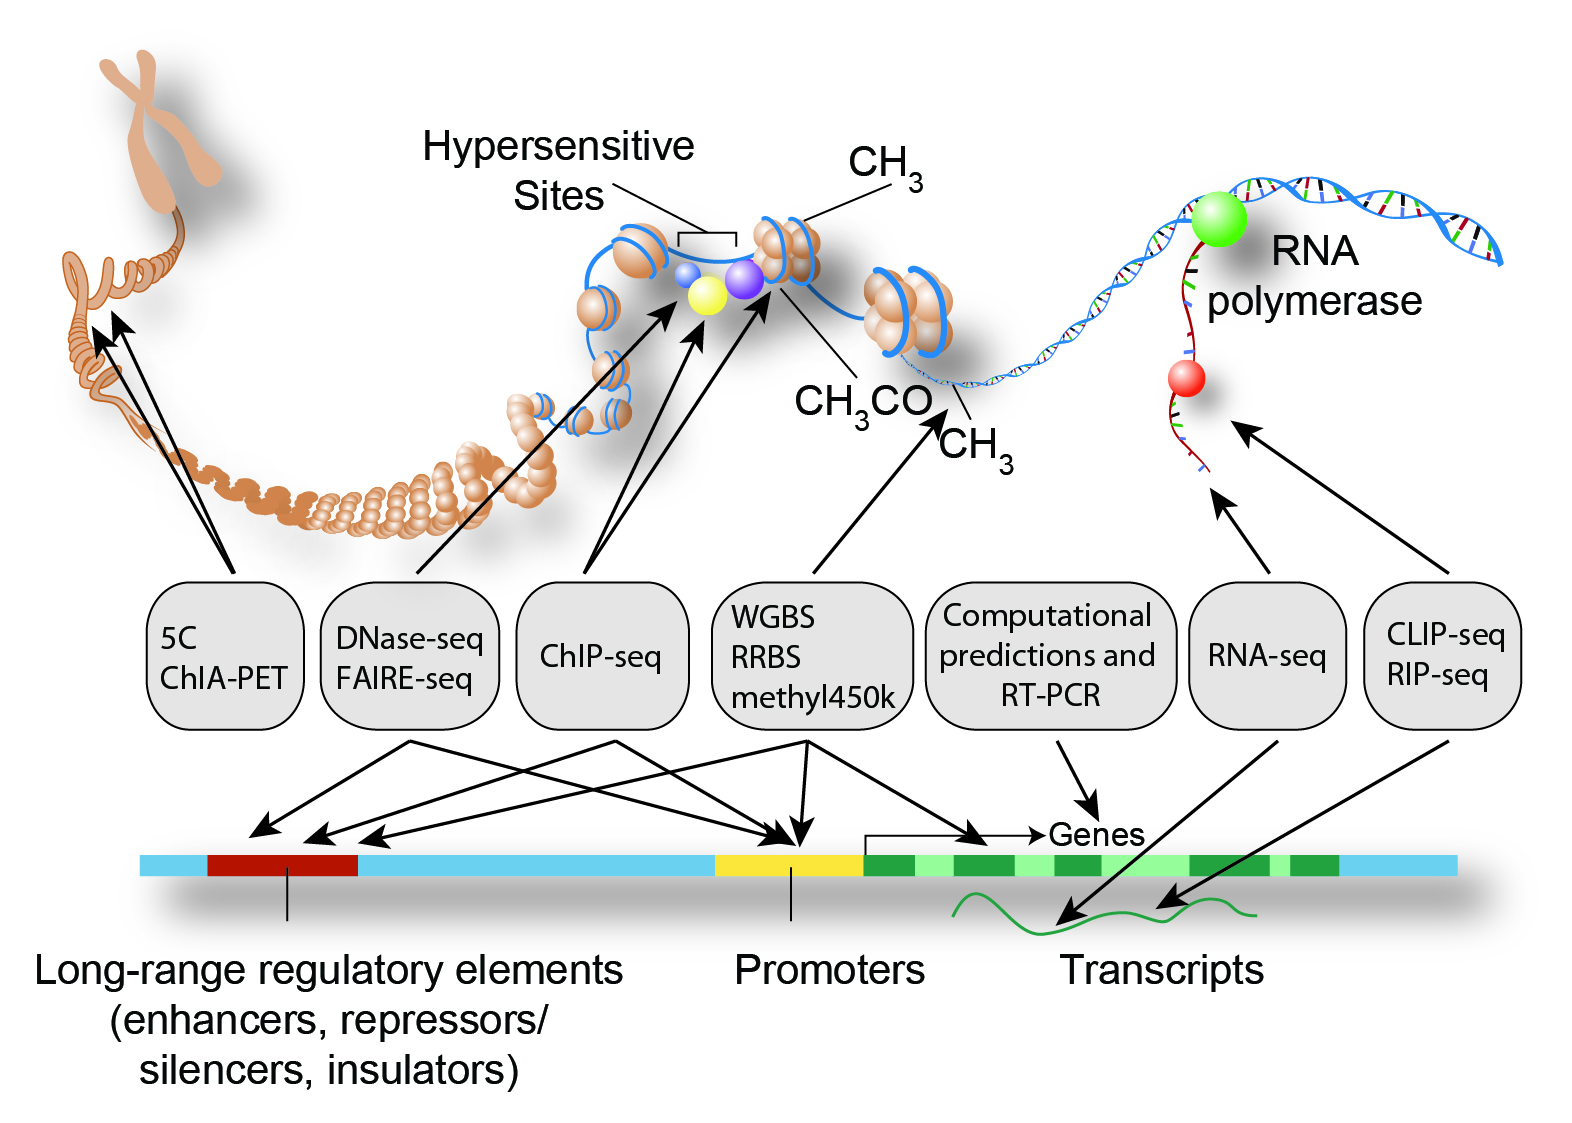
\includegraphics[scale = 0.15]{images/encode-seq.png}
\caption{\emph{Some of the XX-Seq techniques used from the ENCODE projet. Credits: Darryl Leja (NHGRI), Ian Dunham (EBI), Michael Pazin (NHGRI) \citep{Dunham2012}.}}
\label{seq-pic}
\end{center}
\end{figure} 

Recent research studies, assisted by whole-genome data analysis, demonstrated that gene expression and histone modifications (HMs) are well correlated, since a probabilistic model was created, which given a small number of HMs it could predict gene expression \citep{Karlic2010}. Also, \citep{Benveniste2014}, using the richness of the ENCODE datasets \citep{Dunham2012}, learned a logistic regression classifier with the TFs as input features and showed that only from knowledge of TF binding patterns at promoters they could accurately predict HMs. These are only some studies that show the correlation between genetic and epigenetic mechanisms. 

From the aforementioned, it is evident that in order to uncover and interpret the biological regulatory mechanisms an integrative analysis of these heterogeneous biomedical datasets should be performed, since by performing separate analyses of each data source we may not capture important associations between them.
\section{Mixture Models} \label{mixture-models-section}

The aim of this project is focused on modelling and clustering multisource biomedical data. Clustering is a widely used exploratory tool, whose main task is to identify and group similar objects together in \emph{'clusters'}. Clustering can can be categorized as an \emph{unsupervised} learning approach, since we try to discover hidden structure in unlabelled data.     

Different algorithms have been proposed for performing clustering, including hierarchical clustering (agglomerative or top down), k-means \citep{MacQueen1967}, and mixture models \citep{McLachlan1988}. This project is concentrated on \emph{mixture models} which are probabilistic, in the sense that they claim how the data might look like by modelling each cluster by certain probability density functions, \eg mixture of Gaussian distributions.  

A mixture model is a convex combination of two or more probability density functions, possibly of different distributional types. By using a superposition of the individual probability density functions, mixture models are capable of approximating any continuous distribution to arbitrary accuracy \citep{Marin2005}. Mixture models can be formulated as Latent Variable Models (LVMs), where the latent variables have discrete states and can be interpreted as defining assignments of data points to specific components of the mixture model.

Formally, let $x_{i}$, where $i \in \lbrace 1, ... , N \rbrace$, be a given dataset with N objects. The goal of clustering is to partition the objects into at most K clusters. Let $p(x_{i}|\theta)$ be the probability distribution for $x_{i}$ parametrized by $\theta$, $z_{i} \in \lbrace 1,...,K \rbrace$ represent the component that is responsible for $x_{i}$, and $\pi_{k}$ be the probability that an object belongs to cluster $k$, \ie $\pi_{k} = p(z_{i} = k)$. We refer to $\pi_{k}$ as \emph{mixing proportions} and to $z_{i}$ as \emph{latent variables} since they are not observed in the data, but are introduced to allow complicated distributions to be formed from simpler components. 

Thus, the mixture model is defined as follows:
\begin{equation} \label{mix-model-f-mm}
	\begin{aligned}
		p(x_{i}|\Theta) & = \sum_{k=1}^{K} p(z_{i} = k) p(x_{i}|\theta_{k}) \\
			& = \sum_{k=1}^{K}\pi_{k} p(x_{i}|\theta_{k})
	\end{aligned}
\end{equation}
where $\Theta = (\theta_{1},..., \theta_{k}, \pi_{1},..., \pi_{k})$ is the set of all parameters, which must satisfy:
\begin{equation}
		\pi_{k} \in (0, 1) \; \text{for} \; k \in \lbrace 1,...,K \rbrace, \; and 
\end{equation}
\begin{equation}
		\sum_{k=1}^{K}\pi_{k} = 1 
\end{equation}

Mixture models are \emph{generative models}, which means that they give us information for generating new objects. The procedure is the following: first we choose a component, with probabilities given by the mixing proportions, and then we generate an object from the corresponding probability distribution. Formally:
\begin{equation}
	\begin{aligned}
		z_{i} \; & \sim \; Cat(\pi_{1},...,\pi_{K}) \\
		x_{i} | z_{i}=k \; & \sim \; p(x_{i}|\theta_{k})
	\end{aligned}
\end{equation}
where $Cat(\pi_{1},...,\pi_{K})$ is the \emph{categorical} distribution, \ie \emph{multinomial} distribution over a single trial.

\emph{Fig.\ref{gmm-pic}} shows a Gaussian Mixture Model (GMM) with three components in two-dimensional space. It is clear that a single Gaussian distribution would be unable to capture the characteristics of the data since it is unimodal, but a linear superposition of $K$ Gaussian distributions can approximate the continuous density of the data to arbitrary accuracy. 

\begin{figure}[!ht]
	\begin{center}
 		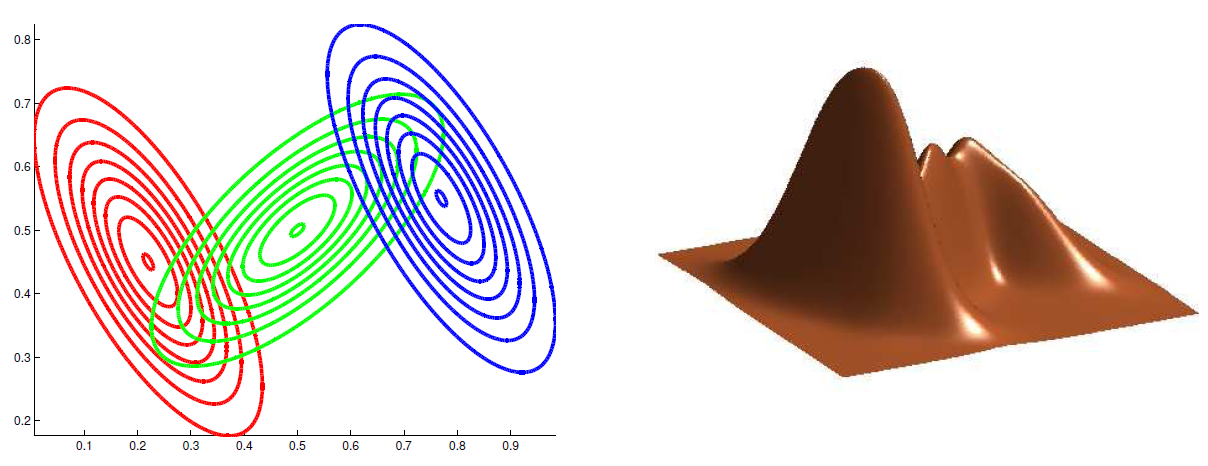
\includegraphics[scale = 0.43]{images/gmm.png}
		 	  \caption{\emph{\textbf{Left:} Contours of constant density for each of the mixture components, where each component is denoted by a different colour. \textbf{Right:} A surface plot of the probability distribution $p(\mathbf{X}|\Theta)$ \cite[Ch. \ 2]{Bishop2006}.}}
		\label{gmm-pic}
	\end{center}
\end{figure}

\subsection{Mixture Model Estimation} \label{mixt-model-estimation-l-subsect}
The model can be fitted to the data using Maximum Likelihood Estimation (MLE). The likelihood is the probability of observing the data given the parameters, and is a function of the parameters. Given a dataset $\mathbf{X}$ consisting of $N$ independent and identically distributed (i.i.d) objects $x_{1}, ..., x_{N}$, the log likelihood function for any mixture model is given by:
\begin{equation} \label{likelihood-f-mm}
	\ell(\Theta) \triangleq p(\mathbf{X}|\Theta) = \sum_{i=1}^{N} \log \bigg\lbrace \sum_{k=1}^{K}\pi_{k}p(x_{i}|\theta_{k})\bigg\rbrace
\end{equation}
The MLE approach is to find the set of parameters $\Theta$ that maximizes \emph{Eq. \ref{likelihood-f-mm}}, that is:
\begin{equation} \label{MLE-f-mm}
	\hat{\Theta} =  \underset{\Theta}{\operatorname{argmax}} \; \ell(\Theta)
\end{equation}

Unfortunately, the presence of the summation inside the logarithm in \emph{Eq. \ref{likelihood-f-mm}} prevents the possibility of deriving an analytical solution. Thus, one should use numerical optimisation procedures, and one of the most widely used algorithms for estimating parameters of mixture models is \emph{Expectation Maximization} (EM) algorithm \citep{Dempster1977}. 
\subsection{The EM algorithm} \label{em-algorithm-l-subsect}
EM is a general iterative algorithm for computing MLEs when there are missing data or latent variables. As aforementioned, mixture models can be formulated as LVMs, thus, EM arises naturally and alternates between inferring the latent values given the parameters (\emph{E-step}), and then optimizing the parameters given the filled in data (\emph{M-step}). EM exploits the fact that if the data were fully observed then the MLE would be easy to compute. In their classic paper \cite{Dempster1977} proved that EM monotonically increases the log likelihood and it converges to a maximum likelihood estimator. The algorithm ends when a convergence criterion is satisfied, \eg the log likelihood does not increase above a certain threshold between two consecutive iterations. 

\emph{Fig. \ref{em-algorithm-pic}} illustrates the EM algorithm for the mixture of two Gaussian distributions applied to the Old Faithful dataset.
\begin{figure}[ht!]
     \begin{center}
        \subfigure[]{
            \label{fig:first}
            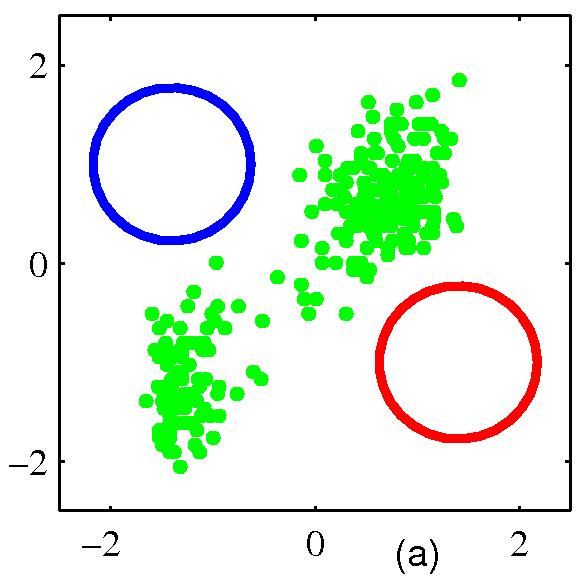
\includegraphics[width=0.3\textwidth]{images/em-a.jpg}
        }
        \subfigure[]{
           \label{fig:second}
           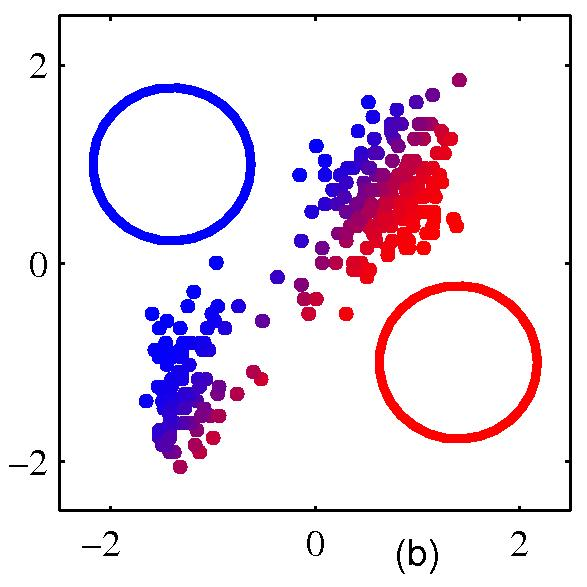
\includegraphics[width=0.3\textwidth]{images/em-b.jpg}
        }
        \subfigure[]{
            \label{fig:third}
            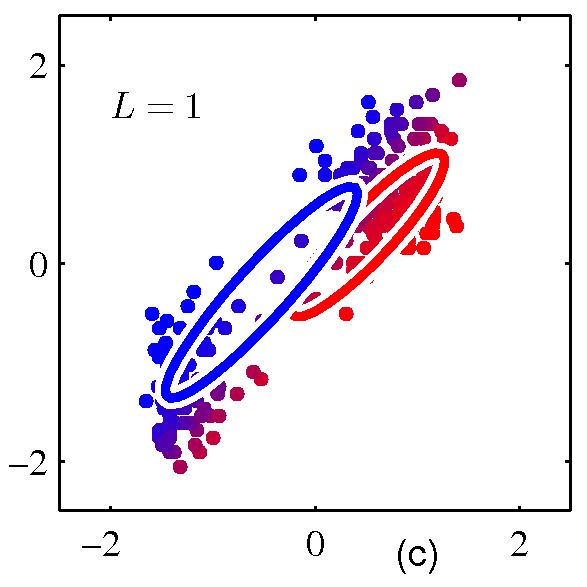
\includegraphics[width=0.3\textwidth]{images/em-c.jpg}
        } %  ------- End of the first row ----------------------%
        \subfigure[]{
            \label{fig:fourth}
            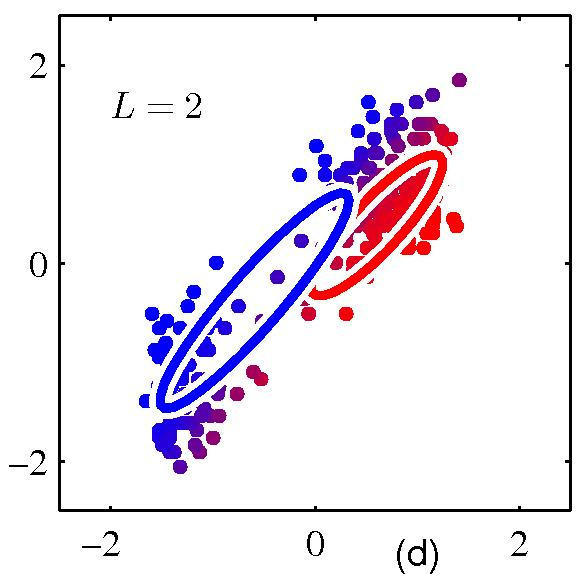
\includegraphics[width=0.3\textwidth]{images/em-d.jpg}
        }
        \subfigure[]{
            \label{fig:fifth}
            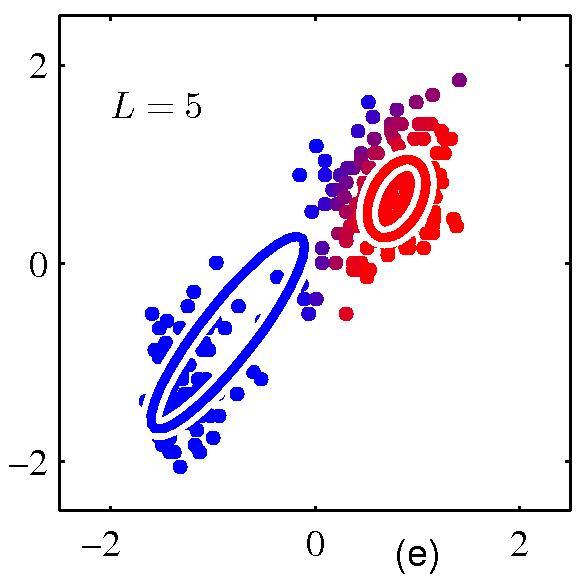
\includegraphics[width=0.3\textwidth]{images/em-e.jpg}
        }
        \subfigure[]{
            \label{fig:sixth}
            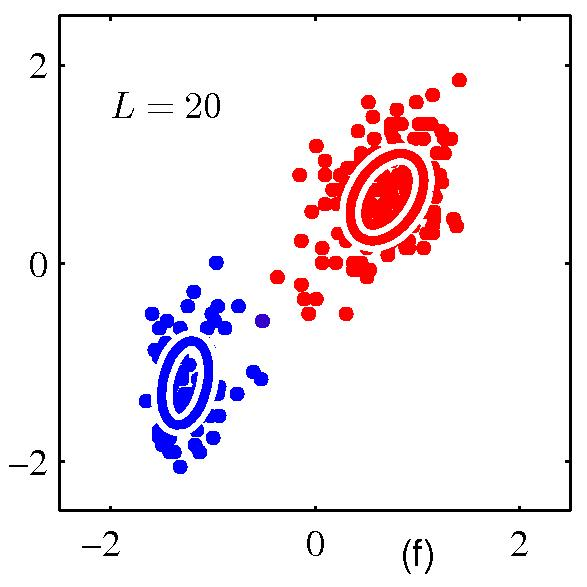
\includegraphics[width=0.3\textwidth]{images/em-f.jpg}
        }
    \end{center}
    \caption{\emph{Illustration of the EM algorithm using the Old Faithful dataset. Plot (a) shows initial parameters. Plots (b) and (c) show the E and M steps in the first iteration, respectively. Plots (d), (e) and (f) show the results after 2, 5 and 20 complete iterations of EM algorithm, respectively. \cite[Ch. \ 9]{Bishop2006}.}}
   \label{em-algorithm-pic}
\end{figure}

Our presentation for the derivation of the EM algorithm is based on \cite[Ch. \ 11]{Murphy2012}.

Let $x_{i}$ be the observed variables, and $z_{i}$ be the hidden or latent variables. We are interested in maximizing the log likelihood of the observed data:
\begin{equation} \label{log-lik-observed-f-mm}
	\ell(\Theta) \triangleq \sum_{i=1}^{N} \log p(x_{i}|\theta) =  \sum_{i=1}^{N} \log \bigg[\sum_{z_{i}} p(x_{i}, z_{i}|\theta) \bigg]
\end{equation}
which is hard to optimize due to the presence of the summation inside the logarithm, so the logarithm no longer acts directly on the likelihood function.

Let us define the \emph{complete data log likelihood} as follows:
\begin{equation} \label{log-lik-comp-observed-f-mm}
	\ell_{c}(\Theta) \triangleq \sum_{i=1}^{N} \log p(x_{i}, z_{i}|\theta)
\end{equation}

If the variables $z_{i}$ were observed, we assume that this likelihood could be easily computed. EM gets around this problem by defining the \emph{expected complete data log likelihood} as:
\begin{equation} \label{log-lik-expected-f-mm}
		Q(\Theta, \Theta^{t-1}) \triangleq \mathbb{E} \big[\ell_{c}(\Theta) | \mathbf{X}, \Theta^{t-1}\big]
\end{equation}
where $t$ is the current iteration. The expectation is taken with respect to the old parameters $\Theta^{t-1}$ and the observed data $\mathbf{X}$. In the \emph{E-step}, we compute the terms inside $Q(\Theta, \Theta^{t-1})$ for which MLE depends on. In the \emph{M-step}, we optimize Q w.r.t $\Theta$:
\begin{equation} \label{max-log-lik-observed-f-mm}
	\Theta^{t} = \underset{\Theta}{\operatorname{argmax}} \; Q(\Theta, \Theta^{t-1})
\end{equation}

For the specific case of mixture models, the expected complete data log likelihood is:
\begin{equation} \label{log-lik-expected-derivation-f-mm}
	\begin{aligned}
		Q(\Theta, \Theta^{t-1}) & \triangleq \mathbb{E} \big[\ell_{c}(\Theta) | \mathbf{X}, \Theta^{t-1}\big] \\
								& = \mathbb{E} \bigg[ \sum_{i} \log p(x_{i}, z_{i}|\theta) \bigg] \\
								& = \sum_{i} \mathbb{E} \bigg[ \log \bigg[\prod_{k} \big( \pi_{k}p(x_{i}|\theta_{k})\big)^{\mathbb{I}(z_{i}=k)} \bigg]\bigg] \\
								& = \sum_{i} \sum_{k} \mathbb{E} \big[\mathbb{I}(z_{i}=k)\big] \log \big[\pi_{k}p(x_{i}|\theta_{k})\big] \\
								& = \sum_{i} \sum_{k} p(z_{i}=k|x_{i},\theta_{k}^{t-1}) \log \big[\pi_{k}p(x_{i}|\theta_{k})\big] \\
								& = \sum_{i} \sum_{k} \gamma(z_{ik}) \log \big[\pi_{k}p(x_{i}|\theta_{k})\big] \\
								& = \sum_{i} \sum_{k} \gamma(z_{ik}) \log \pi_{k} + \sum_{i} \sum_{k} \gamma(z_{ik}) \log p(x_{i}|\theta_{k}) \\		
	\end{aligned}
\end{equation}
where, $\gamma(z_{ik}) \triangleq p(z_{i}=k|x_{i},\theta_{k}^{t-1})$ is the responsibility that component k takes for explaining the observation $x_{i}$, and $\mathbb{I}(z_{i}=k)$ is an indicator function, equal to 1 if $z_{i}=k$, and 0 otherwise.


\subsubsection{E-Step}
The E-step can be computed using the following form for any mixture model, which is the responsibility that component k takes for explaining the observation $x_{i}$:
\begin{equation} \label{responsibilities-f-mm}
  \begin{aligned}
	\gamma(z_{ik}) & \triangleq p(z_{i}=k|x_{i},\theta_{k}^{t-1}) \\
				   & = \frac{p(z_{i}=k)p(x_{i}|z_{i}=k,\theta_{k}^{t-1})}{\sum\limits_{j=1}^{K} p(z_{i}=j)p(x_{i}|z_{i}=j,\theta_{j}^{t-1})} \\
				   & = \frac{\pi_{k}p(x_{i}|z_{i}=k,\theta_{k}^{t-1})}{\sum\limits_{j=1}^{K} \pi_{j}p(x_{i}|z_{i}=j,\theta_{j}^{t-1})}
  \end{aligned}
\end{equation}


\subsubsection{M-Step}
In the M-step we optimize $Q$ with respect to parameters $\Theta = (\theta_{1},...,\theta_{K},\pi_{1},...,\pi_{K})$.

For the mixing proportions $\pi_{k}$, we take the derivative of \emph{Eq. \ref{log-lik-expected-derivation-f-mm}} w.r.t. $\pi_{k}$ and set it to zero; due to the constraint that $\sum_{k=1}^{K}\pi_{k} = 1$ we introduce a Lagrange multiplier. Thus we have:

\begin{equation} \label{derivative-mix-prop-f-mm}
  \begin{aligned}
	\frac{\partial}{\partial \pi_{k}} \bigg[  Q(\Theta, \Theta^{t-1}) + \lambda \big( \sum_{k}\pi_{k} - 1\big) \bigg] & = 0 \\
	\sum_{i} \frac{1}{\pi_{k}} \gamma(z_{ik}) + \lambda & = 0 
  \end{aligned}
\end{equation}
Setting $\lambda = - N$, the result, which is the same for any mixture model, is:
\begin{equation} \label{mixing-proportions-est-f-mm}
		\pi_{k} = \frac{1}{N} \sum_{i} \gamma(z_{ik})
\end{equation}

To derive the M-step for the parameters $\theta_{k}$, we only need to keep the terms of \emph{Eq. \ref{log-lik-expected-derivation-f-mm}} that depend on $\theta_{k}$, that is:
\begin{equation} \label{parameters-est-EM-M-f-mm}
		\ell(\theta_{k}) \triangleq \sum_{i} \sum_{k} \gamma(z_{ik}) \log p(x_{i}|\theta_{k})
\end{equation}
and we optimize them with respect to $\theta_{k}$.

The maximization of \emph{Eq. \ref{parameters-est-EM-M-f-mm}} yields different results depending on the probability distribution $p(x_{i}|\theta_{k})$. For most of the well known probability distributions, including the Normal, Binomial, Poisson, etc., direct maximization of $\ell(\theta_{k})$ is feasible. 

For more complex likelihood functions, the maximization of $\ell(\theta_{k})$ may be intractable, thus numerical optimization strategies \citep{Nocedal2006}, such as conjugate gradients algorithm \citep{Hestenes1952} should be exploited. This extension of EM algorithm is known as \emph{Generalised EM}, or GEM, and it has been proved that on each EM iteration of the GEM algorithm the log likelihood increases, and thus converges to the maximum likelihood estimate \citep{Wu1983}.
\section{Hierarchical Bayesian Mixture Models} \label{fdmm-s}

\subsection{Bayesian Statistics}
The use of Maximum Likelihood for inferring the values of the parameters $\Theta$ belongs in the \emph{frequentist} interpretation of probability. In this approach, the parameters $\Theta$ are considered to be fixed, the values are inferred by an estimator, \eg MLE, and we get error bars for the estimates by considering a distribution over datasets $\mathbf{X}$ \cite[Ch. 1]{Bishop2006}. 

On the other hand, in Bayesian statistics, probabilities provide a quantification of uncertainty or degrees of belief supported by the available evidence. In this setting, the dataset $\mathbf{X}$ is observed and hence is fixed, and we express our uncertainty in the model parameters, by considering the parameters themselves as random variables. Our initial beliefs about $\Theta$, before observing the data, are represented by a \emph{prior} probability distribution $p(\Theta)$. The effect of observing the data $\mathbf{X}$ is given through the \emph{likelihood} function $p(\mathbf{X}|\Theta)$, which is also referred to as the observation model.  The likelihood function expresses how probable are the observed data given the parameters, and is a function of the parameters. Hence, to update our beliefs about the value of $\Theta$, after observing the data $\mathbf{X}$, we use the machinery of probability theory, and more specifically Bayes' theorem, to evaluate the \emph{posterior} probability distribution:

\begin{equation}
  \begin{aligned}
	p(\Theta | \mathbf{X}) & = \frac{p(\mathbf{X}|\Theta) p(\Theta)}{p(\mathbf{X})} \\
	& = \frac{p(\mathbf{X}|\Theta) p(\Theta)}{\int p(\mathbf{X}|\Theta) p(\Theta) d\Theta}
  \end{aligned}
\end{equation}
which can be interpreted as follows:
\begin{equation}
	\text{posterior} = \frac{likelihood \times prior}{evidence}
\end{equation}

For completeness, below are shown the main approaches for parameter estimation.

\subsubsection*{ML Estimation of $\Theta$}
Under the Maximum Likelihood approach we seek the value of $\Theta$ that maximizes the likelihood, that is:
\begin{equation} \label{MLE-f-bayes}
	\hat{\Theta} =  \underset{\Theta}{\operatorname{argmax}} \; p(\mathbf{X}|\Theta)
\end{equation}

\subsubsection*{MAP Estimation of $\Theta$}
Under the Maximum a Posteriori approach we seek the value of $\Theta$ that maximizes the posterior $p(\Theta | \mathbf{X})$, that is:
\begin{equation} \label{MAP-f-bayes}
  \begin{aligned}
	\hat{\Theta} & =  \underset{\Theta}{\operatorname{argmax}} \; p(\Theta | \mathbf{X}) \\
	& \propto \underset{\Theta}{\operatorname{argmax}} \; p(\mathbf{X}|\Theta) p(\Theta)
  \end{aligned}
\end{equation}
where the evidence $p(\mathbf{X})$ can be ignored since it does not depend on $\Theta$. Thus, MAP estimation, in contrast to ML, incorporates in the model our prior beliefs regarding the values of the parameters.

\subsubsection*{Bayesian Estimation of $\Theta$}
Under a full Bayesian approach we compute the posterior distribution over the parameters, that is:
\begin{equation} \label{posterio-f-bayes}
  \begin{aligned}
	p(\Theta | \mathbf{X}) = \frac{p(\mathbf{X}|\Theta) p(\Theta)}{p(\mathbf{X})} 
  \end{aligned}
\end{equation}

Thus, in the Bayesian  instead of estimating a fixed value for the parameters, we also capture the uncertainty of the estimation by computing the posterior distribution of the parameters. On the other hand, i\eg ML or MAP estimations involve in finding an optimum point estimate of the parameters, but they do not account for any uncertainty in the estimated value of the parameters. 

\subsection{Approximate Inference}
Even though Bayesian framework is appealing, it is limited by practical difficulties since we need to marginalize over the whole parameter space, in order to compute the posterior. In most cases marginalization is computationally difficult since the integral might be intractable and difficult to approximate. To be able to compute some of the Bayesian integrals analytically, \emph{conjugate priors} should be used if possible. For a given functional form of the likelihood $p(\mathbf{X}|\Theta)$, the prior $p(\Theta)$ is said to be conjugate for that likelihood, if the posterior $p(\Theta|\mathbf{X})$ has the same functional form as the prior.

When the posterior is intractable to compute, we need to resort to approximation schemes, and these fall broadly into two main classes. Deterministic approximation schemes, such as \emph{Variational Bayes} \citep{Beal2003}, are based on picking an approximation $q(\Theta|\mathbf{X})$ from some tractable family, \eg Gaussian, and then try to make this approximation as similar as possible to the true posterior distribution $p(\Theta|\mathbf{X})$, using a cost function such as KL-divergence \cite[Ch. 21]{Murphy2012}. Thus, Variational Bayes can be seen as an extension of EM algorithm for full Bayesian parameter estimation, since it constructs a lower bound on the marginal likelihood, and attempts to optimise this bound using an iterative scheme \citep{Beal2003}.



\subsection{Finite Dirichlet Mixture Models}
In a Bayesian framework, the parameters themselves are considered as random variables, thus prior distributions need to be placed over these parameters. If possible, conjugate priors should be used.

 

\begin{minipage}{0.6\textwidth}%
  \hfill
  \begin{center}
	% model_pca.tex
%
% Copyright (C) 2012 Jaakko Luttinen
%
% This file may be distributed and/or modified
%
% 1. under the LaTeX Project Public License and/or
% 2. under the GNU General Public License.
%
% See the files LICENSE_LPPL and LICENSE_GPL for more details.

% PCA model

%\beginpgfgraphicnamed{model-pca}
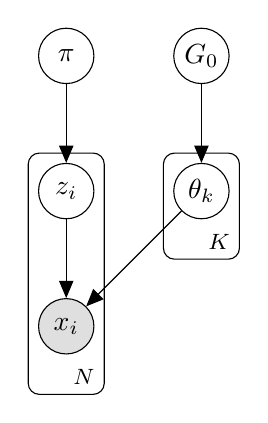
\begin{tikzpicture}

  % Define nodes
  \node[obs]                    (X) {$x_{i}$};
  \node[latent, above=of X] 	(Z) {$z_{i}$};
  \node[latent, above=of Z]  	(p) {$\pi$};
  \node[latent, right=1cm of Z] (t) {$\theta_{k}$};
  \node[latent, above=of t] 	(G) {$G_{0}$};

  % Connect the nodes
  \edge {Z,t} {X} ; %
  \edge {p} {Z} ; %
  \edge {G} {t} ; %

  % Plates
  \plate {} {(t)} {$K$};
  \plate {} {(Z)(X)} {$N$};

\end{tikzpicture}
%\endpgfgraphicnamed

%%% Local Variables: 
%%% mode: tex-pdf
%%% TeX-master: "example"
%%% End: 

	\emph{Graphical Model of FDMM.}
  \end{center}
\end{minipage}
%\hfill
\begin{minipage}{0.1\textwidth}%\raggedright
  \begin{equation*}
  	\begin{aligned}
  		\mathbf{\pi} \; & \sim \; Dir(\mathbf{\delta}) \\
  		z_{i}|\mathbf{\pi} \; & \sim \; Cat(\mathbf{\pi}) \\
  		\theta_{k} \; & \sim \mathcal{G}_{0}; \mathcal{H} \\
  		x_{i}|z_{i}=k,\theta_{k} \; & \sim \; p(\cdot | \theta_{k})  
  	\end{aligned} 
  \end{equation*} 
\end{minipage}

\vspace*{5mm}
The full joint distribution of the FDMM model by looking at the graphical representation factorizes as follows:
\begin{equation}%\scriptstyle
	p(\mathbf{X},\mathbf{Z},\mathbf{\pi},\Theta;\delta,\mathcal{H}) = p(\mathbf{X}|\mathbf{Z},\Theta) p(\mathbf{Z}|\pi) p(\pi|\delta) p(\Theta |\mathcal{G}_{0}; \mathcal{H})
\end{equation}

where $\mathcal{H}$ is the set of all the hyper-parameters of the $\mathcal{G}_{0}$ prior distribution related to the parameters $\Theta$, and $\mathbf{\delta}$ is a K-dimensional vector with the hyper-parameters of the \emph{Dirichlet} prior. 

To do inference in the Bayesian framework, the posterior distribution of the parameters needs to be computed. By applying the Bayes Rule and conditioning on the observed data $\mathbf{X}$, the posterior distribution is simply proportional to the full joint. Thus:
 
\begin{equation}%\scriptstyle
  \begin{aligned}
	p(\mathbf{Z},\mathbf{\pi},\Theta|\mathbf{X} ;\delta,\mathcal{H}) & = \frac{p(\mathbf{X}|\mathbf{Z},\mathbf{\pi},\Theta) p(\mathbf{Z},\mathbf{\pi},\Theta ;\delta,\mathcal{H})}{p(\mathbf{X})} \\
	   & \propto p(\mathbf{X}|\mathbf{Z},\mathbf{\pi},\Theta) p(\mathbf{Z},\mathbf{\pi},\Theta ;\delta,\mathcal{H}) \\
	   & = p(\mathbf{X}|\mathbf{Z},\Theta) p(\mathbf{Z}|\pi) p(\pi|\delta) p(\Theta |\mathcal{G}_{0}; \mathcal{H}) \\
	   & = \bigg(\prod\limits_{i=1}^{N} p(x_{i}|z_{i},\theta_{z_{i}}) p(z_{i}|\pi)\bigg) p(\pi|\delta) \bigg(\prod\limits_{k=1}^{K} p(\theta_{k} |\mathcal{G}_{0}; \mathcal{H})\bigg)
  \end{aligned}
\end{equation}
where we use the fact that $\mathbf{X}$ is conditionally independent of $\pi$ given $\mathbf{Z}$, \ie $\mathbf{X} \bigCI \pi \;| \; \mathbf{Z} $. 


Deriving Gibbs sampler for this model requires deriving an expression for the conditional distribution of every random variable conditioned on all the others. More specifically, for the FDMM we have the following quantities:
\begin{equation}%\scriptstyle
	p(\mathbf{\pi}|\mathbf{X},\mathbf{Z},\Theta;\delta,\mathcal{H}) = p(\mathbf{\pi} | \mathbf{Z};\delta) \sim Dir(\delta + N_{k})
\end{equation}

\begin{equation}%\scriptstyle
	p(\mathbf{\Theta}|\mathbf{X},\mathbf{Z},\pi;\delta,\mathcal{H}) = p(\mathbf{\Theta}|\mathbf{X},\mathbf{Z};\mathcal{H}) \sim \mathcal{G}_{0}(\cdot|\mathcal{H})
\end{equation}

\begin{equation}%\scriptstyle
	p(\mathbf{Z}|\mathbf{X},\mathbf{\Theta},\pi;\delta,\mathcal{H}) = p(\mathbf{\Theta}|\mathbf{X},\mathbf{Z};\mathcal{H}) \sim \mathcal{G}_{0}(\cdot|\mathcal{H})
\end{equation}
\chapter{Next Generation Sequencing Data} \label{dataset-chapter}

\section{ENCODE data} \label{encode-data-sect}
The Encyclopedia of DNA Elements (ENCODE) project \citep{Dunham2012} is an international collaboration of research groups with diverse backgrounds and expertise in production and analysis of NGS genomic data. \emph{Fig. \ref{encode-seq-pic}} shows only some examples of the different platforms and techniques that are used from ENCODE to measure diverse biological components in order to interpret the human genome. That is, to discover functional elements in the genome, including genes, transcripts, transcriptional regulatory regions, chromatin structure and DNA methylation patterns.

\begin{figure}[!ht]
\begin{center}
 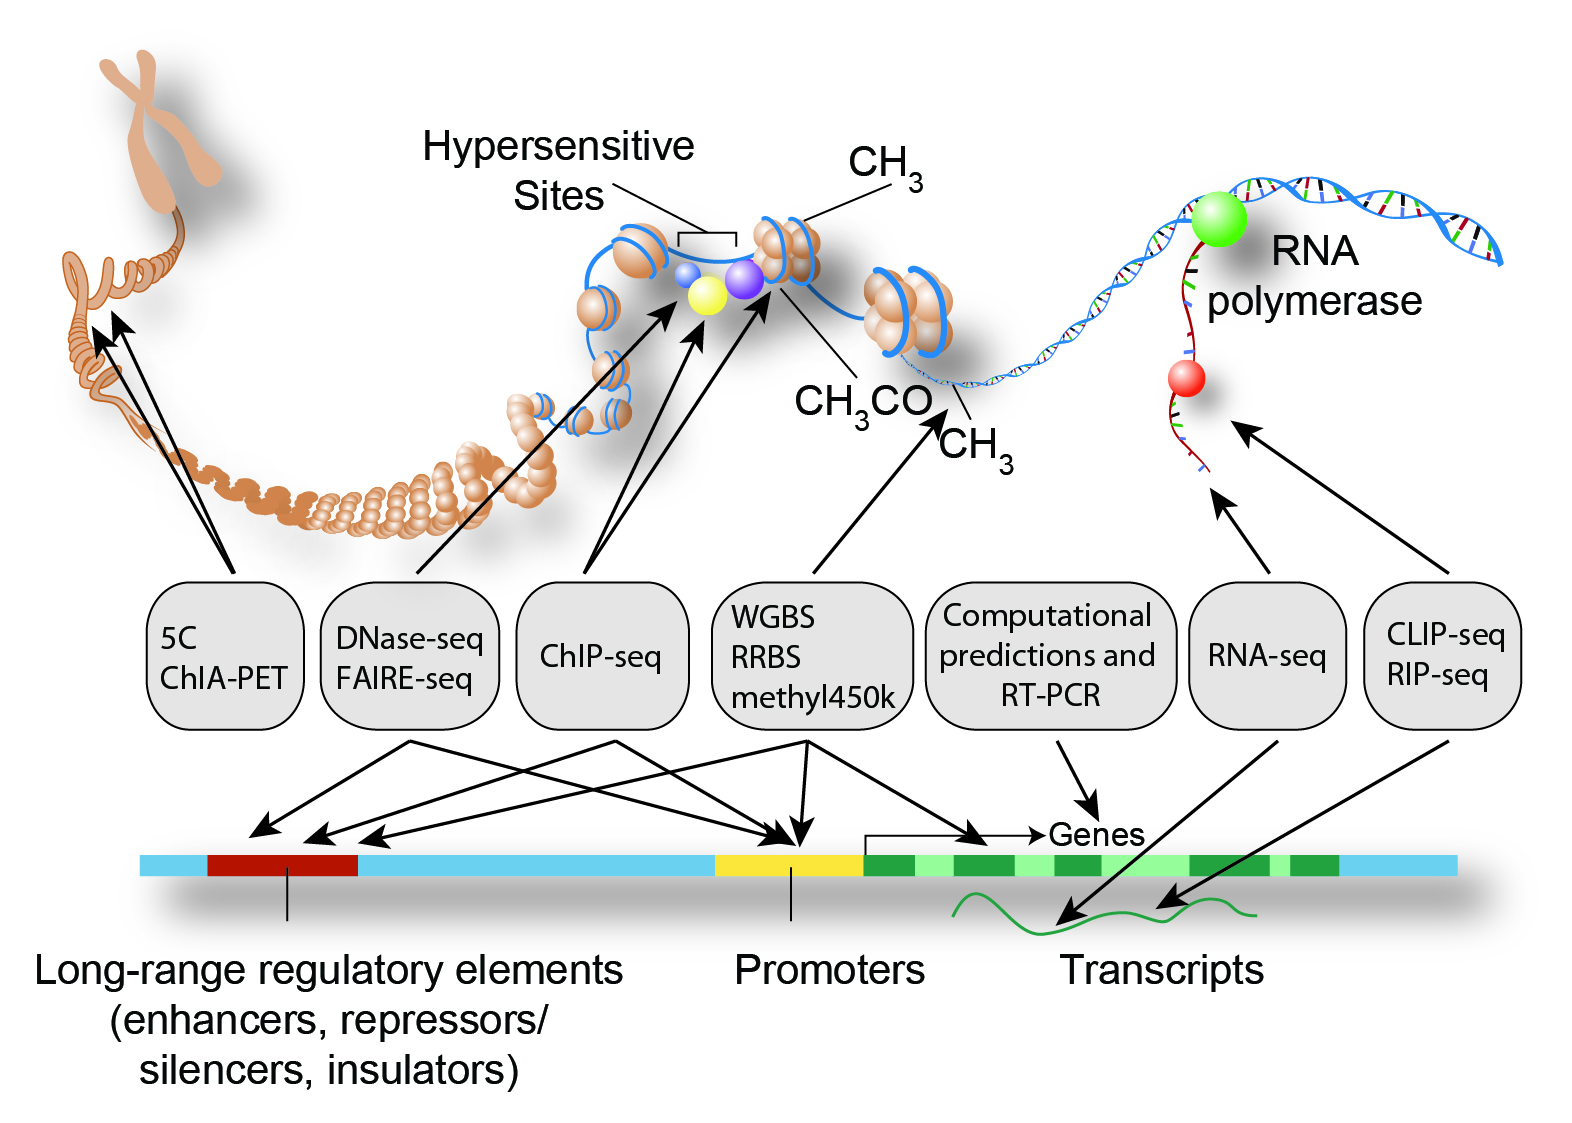
\includegraphics[scale = 0.25]{images/encode-seq.png}
\caption{\emph{Some of the XX-Seq techniques used from the ENCODE projet. Credits: Darryl Leja (NHGRI), Ian Dunham (EBI), Michael Pazin (NHGRI) \citep{Dunham2012}.}}
\label{encode-seq-pic}
\end{center}
\end{figure} 

To evaluate our proposed methods, Tier 1 cells (\ie high priority) from the ENCODE project are used. These data are released to the public through a web accessible database (\emph{http://genome.ucsc.edu/ENCODE/}) and can be visualised through the \emph{UCSC Genome Browser} at the same web portal. More specifically, the cell types that will be studied are the immortalized cell lines, K562, coming from a human female with chronic myelogenous leukemia, and the human embryonic stem cells, H1-hESC, coming from a human male \citep{Dunham2012}.

%This project is mainly concentrated in modelling and analysing transcriptome and DNA methylation data generated from NGS technology.
\subsection{DNA methylation data} \label{dna-methylation-data-sect}
DNA methylation is a well studied chemical modification of DNA, which occurs when a methyl group is attached to a DNA nucleotide. It is associated with diverse biological processes of direct clinical relevance, including gene and transposon silencing, X-chromosome inactivation, and  genomic imprinting \citep{Li1993, Mohandas1981}. In mammals,  methylation is observed almost exclusively on cytosine residues in the context of CpG dinucleotides (\ie C followed by G, where p stands for the phosphate group linking C and G). DNA methylation is said to be a true \emph{epigenetic modification}, since its mechanism of inheritance during the cell cycle is well established \citep{Law2010}. 

Due to the increased vulnerability of the 5-Methylcytosines to randomly deaminate to thymine, most of the genome is depleted from CpG dinucleotides \citep{Scarano1967}, except from small regions, termed \emph{CpG islands} \citep{Bird2002}. A CpG island (CGI) is a sequence of at least 200 bp long, with a greater number of CpG sites than expected from its GC content. These regions are often GC rich, typically unmethylated, and are found upstream of many mammalian genes \citep{Law2010}. 

Bisulphite (or bisulfite) treatment \citep{Frommer1992} followed by NGS can be used to measure the methylation level of the genomic DNA at a single-nucleotide resolution, and is termed Whole-Genome Bisulphite Sequencing (WGBS). Sodium bisulphite efficiently deaminates unmethylated cytosines to uracils, and leaves the 5-Methylcytosines unchanged. Uracils are read as thymines by DNA polymerase, thus when amplifying the data during PCR (Polymerase Chain Reaction), the unmethylated cytosines appear as thymines \citep{Krueger2012}. Reads are then aligned to a reference genome allowing changes of C to T during the mapping procedure. 
The outline of the bisulphite treatment of a sample DNA sequence is shown in \emph{Fig. \ref{bisulphite-pic}}.
\begin{figure}[!ht]
	\begin{center}
 		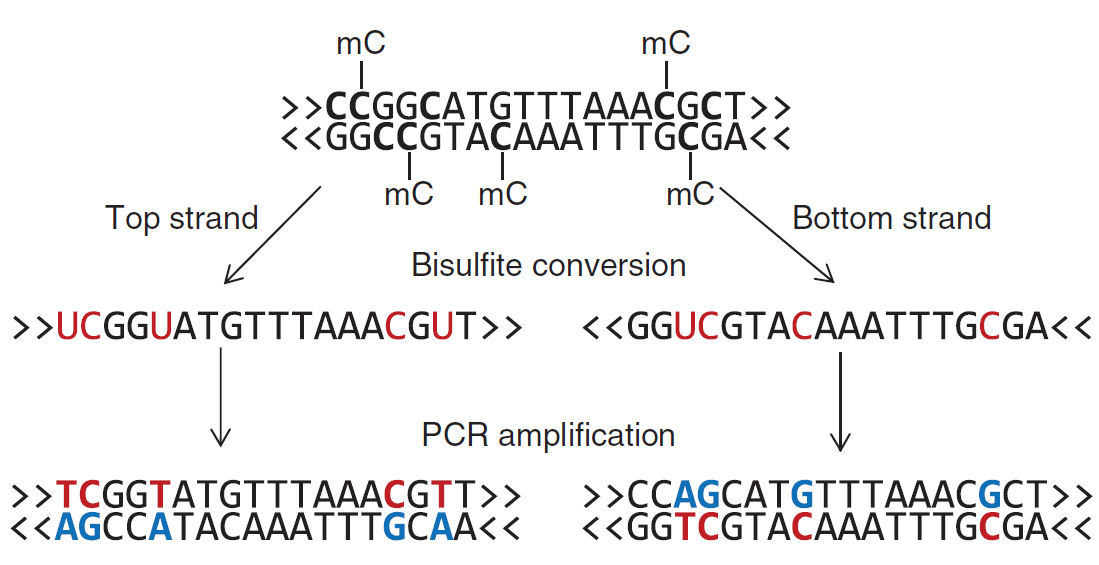
\includegraphics[scale = 0.4]{images/bis-treatment.png}
		\caption{\emph{Outline of the bisulphite treatment and subsequent PCR amplification of a sample DNA sequence. Unmethylated cytosines are deaminated to uracils by bisulphite, while 5-Methylcytosines are resistant to conversion \citep{Krueger2012}.}}
		\label{bisulphite-pic}
	\end{center}
\end{figure} 

In WGBS experiments, the DNA molecules often originate from distinct cells, as a consequence, the methylation state of a particular cytosine may be different across DNA molecules. Hence, in the context of WGBS experiments the methylation of a particular cytosine is described as \emph{methylation level}, which is the fraction of the molecules in the sample containing 5-Methylcytosines at the specific genomic locus \citep{Schultz2012}. \emph{Read coverage} is the average number of times a CpG site is read during the sequencing process, and depends on the sequencing depth.

\cite{Meissner2005} developed a technique, termed Reduced Representation Bisulphite Sequencing (RRBS), for analyzing the genome-wide methylation profiles efficiently, at lower cost and with greater coverage of CpG dense regions. This method combines bisulphite treatment and restriction enzymes, such as MspI, to generate a \emph{reduced representation} of the genome of a strain, tissue or cell type which have a high CpG content \citep{Meissner2005}. 

%For the purpose of this project, RRBS data from the H1-hESC and K562 cells will be analysed. Both datasets were generated by the Myers Lab at the HudsonAlpha Institute for Biotechnology. 
%\chapter{Mixture Modelling of DNA Methylation Profiles} \label{model-meth-chapter}

\section{Introduction} \label{motivation-meth-l}
DNA methylation data generated from NGS provide us with the methylation level of the genomic DNA at each cytosine. But, what is often of practical interest is identifying the methylation profile of a genomic region, \eg the methylation profile of a promoter. \cite{Vanderkraats2013} suggested that the shape of the methylation profile plays an important role in predicting gene expression, leading to a potentially functional role for methylation patterns. This means that higher-order properties, such as shape, of the methylation profiles over a region should be considered. Taking into consideration that the methylation level of a CpG site is highly correlated with the methylation level of the surrounding CpGs (\ie spatial co-dependence), \cite{Mayo2014} developed M$^3$D, which is non-parametric kernel-based method for statistical identification of differentially methylated regions (DMRs). This project makes the same assumption about the \emph{spatial co-dependence} of CpGs, but is mainly concentrated in clustering together similar methylation profiles.
\section{Modelling DNA Methylation Profiles} \label{model-meth-profiles-s}
The measurement process of DNA methylation can be modelled with a Binomial distribution. Assume that \emph{t} is the total number of reads that are mapped to a specific CpG site, and that the 5-Methylcytosine were found in \emph{m} of these reads. Then for each CpG site we have the read proportion \emph{(m,t)}, and we assume that:
\begin{equation} \label{binom-1d-f-meth}
	m \sim Binom(t, p)
\end{equation}
where \emph{p} is the unknown methylation level of the CpG site.

We are interested in modelling methylation profiles across different genomic regions, \eg promoter regions, hence the data can be represented as a set of vectors, whose dimensionality \emph{L} depends on the number of the individual CpG sites for that specific region. Formally, each region \emph{i} can be represented by a vector $\mathbf{y}_{i}$ of dimensionality $L_{i}$, and each entry of the vector consists of the tuple:
\begin{equation}
	%n_{i}^{l} = \frac{m_{i}^{l}}{t_{i}^{l}}
	y_{il} = (m_{il},t_{il})
\end{equation}
where, $m_{il}$ is the number of 5-Methylcytosine reads on $l$-th CpG site in region $i$, and $t_{il}$ is the total number of reads on $l$-th CpG site in region $i$. 

Hence, we can formulate our problem as a \emph{regression} problem, where we try to fit a function $\mathbf{f}$, of some specific form, to the observations $\mathbf{y}$. A promising approach for modelling the methylation profile for a given region is to use a \emph{Gaussian Process} for classification \citep{Rasmussen2006}. Even though this approach would be ideal, its time complexity of $O(n^{3})$ is prohibitive for our purposes. A computationally more attractive approach would be to follow a parametric approach by selecting an explicit set of basis functions.

More specifically, let $\mathbf{x}_{i}$ be the genomic region of interest, $\mathbf{y}_{i}$ be the vector of observations in this region (\ie proportions of methylated reads to the total reads at each site), and let $f(\mathbf{x}_{i})$ be a latent function representing the methylation profile at that specific genomic region. Since the observed methylation data are actually the fraction of total reads that contained methylated cytosines, each entry in the region will take values in the $[0, 1]$ interval, thus, we introduce a latent function $g(\mathbf{x}_{i})$, \eg $g(\mathbf{x}_{i}) = \alpha \mathbf{x}_{i}^{2} + \beta \mathbf{x}_{i} + c$, defined as the \emph{inverse probit transformation} of $f(\mathbf{x}_{i})$. In other words, $f(\mathbf{x}_{i})$ is the probit transformation of $g(\mathbf{x}_{i})$:
\begin{equation} \label{probit-transform-f-meth}
	f(\mathbf{x}_{i}) = \Phi(g(\mathbf{x}_{i}))
\end{equation}
where $\Phi(x)$ is the Cumulative Distribution Function (CDF) of the standard normal distribution:
\begin{equation} \label{cdf-stand-normal-f-meth}
	\Phi(x) = \frac{1}{\sqrt{2\pi}} \int_{-\infty}^{x} e^{-t^{2}/2}dt
\end{equation}

Let $\mathbf{f}_{i} = f(\mathbf{x}_{i})$ and $\mathbf{g}_{i} = g(\mathbf{x}_{i})$ be shorthand for the values of the latent functions.

Given the values of the latent function $\mathbf{f}_{i}$, the observations at each CpG site for that region are independent Binomial variables, as shown in \emph{Eq. \ref{binom-1d-f-meth}}, so the joint likelihood factorizes and we have:
\begin{equation} \label{likel-binom-prob-f-meth}
  \begin{split}
	p(\mathbf{y}_{i}|\mathbf{f}_{i}) & = \prod_{l=1}^{L} p(y_{il}|f_{il}) \\
							 & = \prod_{l=1}^{L} Binom(t_{il}, f_{il}) \\
							 & = \prod_{l=1}^{L} Binom\big(t_{il}, \Phi(g_{il})\big) \\
							 & = \prod_{l=1}^{L} \binom{t_{il}}{m_{il}} \Phi(g_{il})^{m_{il}} (1 - \Phi(g_{il})\big)^{t_{il} - m_{il}}
  \end{split}
\end{equation}

From its final form, we refer to this function as the \emph{Binomial distributed Probit regression function}. In practice, the likelihood is computed in the log space, due to numerical issues when multiplying many probabilities of small numbers leading to underflow errors. Thus, the joint log likelihood for region \emph{i} is:
\begin{equation} \label{likel-binom-prob-log-f-meth}
  \begin{split}
	\log p(\mathbf{y}_{i}|\mathbf{f}_{i}) & = \sum_{l=1}^{L} \log p(y_{il}|f_{il}) \\
				& = \sum_{l=1}^{L} \log \bigg(\binom{t_{il}}{m_{il}} \Phi(g_{il})^{m_{il}} \big(1 - \Phi(g_{il})\big)^{t_{il} - m_{il}}\bigg) \\
				& = \sum_{l=1}^{L} \bigg(\log \binom{t_{il}}{m_{il}} + m_{il} \log \Phi(g_{il}) + \big(t_{il} - m_{il} \big) \log \big(1 - \Phi(g_{il})\big)\bigg)
  \end{split}
\end{equation}
\section{Clustering DNA Methylation Profiles} \label{cluster-meth-s}
After defining a model for the DNA methylation profiles, a statistical method needs to be proposed in order to perform model-based clustering of methylation profiles. 

A mixture model approach \citep{McLachlan1988} is chosen to cluster methylation profiles, and the model is fitted to the data using maximum likelihood. Thus, \emph{EM algorithm} \citep{Dempster1977} is chosen to estimate the mixture model parameters. Below we derive the \emph{E} and \emph{M} steps for clustering methylation profiles using the \emph{Binomial distributed Probit regression function} as the observation model. 

But before, we have to explicitly introduce the parameters $\theta_{k}$ of the observation model, excluding the mixing proportions $\pi_{k}$ which are present for any mixture model. For example, in a Gaussian Mixture Model (GMM) the model parameters $\theta_{k}$ are the mean $\mu_{k}$ and the variance $\sigma_{k}^{2}$ of the Gaussian components. In our model, the Binomial distributed Probit regression function, the parameters are the coefficients of the $n^{th}$ degree polynomial function $\mathbf{g}_{i}$. Thus, during the EM algorithm we infer these sets of parameters for each cluster $k$. 

For example, for a $2^{nd}$ degree polynomial, we can rewrite \emph{Eq. \ref{likel-binom-prob-f-meth}} by explicitly showing the model parameters as follows:
\begin{equation} \label{likel-binom-prob-example1-f-meth}
  \begin{split}
	p(\mathbf{y}_{i}|\mathbf{f}_{i}, \theta) & = \prod_{l=1}^{L} p(y_{il}|f_{il}, \theta) \\
							 & = \prod_{l=1}^{L} Binom \big(t_{il}, \Phi(g_{il}; \theta)\big) \\
							 & = \prod_{l=1}^{L} \binom{t_{il}}{m_{il}} \Phi(\alpha x_{il}^{2} + \beta x_{il} + c)^{m_{il}} (1 - \Phi(\alpha x_{il}^{2} + \beta x_{il} + c)\big)^{t_{il} - m_{il}}
  \end{split}
\end{equation}
where $\theta = (\alpha, \beta, c)$.

\subsection{E-step}
In the E-step we compute the responsibility that component k takes on explaining observations $\mathbf{y}_{i}$, and by substituting the proposed likelihood function to \emph{Eq. \ref{responsibilities-f-mm}}, we have:
\begin{equation} \label{responsibilities-binom-prob-model-f-meth}
  \begin{split}
	\gamma(z_{ik}) & \triangleq p(z_{i}=k|\mathbf{y}_{i},\theta_{k}) \\
				   & = \frac{\pi_{k}p(\mathbf{y}_{i}|\mathbf{f}_{i},z_{i}=k,\theta_{k})}{\sum\limits_{j=1}^{K} \pi_{j}p(\mathbf{y}_{i}|\mathbf{f}_{i},z_{i}=j,\theta_{j})} \\
				   & = \frac{\pi_{k} \prod\limits_{l=1}^{L} Binom \big(t_{il}, \Phi(g_{il}; \theta_{k})\big)} {\sum\limits_{j=1}^{K} \pi_{j} \prod\limits_{l=1}^{L} Binom \big(t_{il}, \Phi(g_{il}; \theta_{j})\big)}
  \end{split}
\end{equation}
Thus, the E-step essentially remains the same, with the difference that at each iteration we need to evaluate pointwise a different observation model. 

\subsection{M-step}
In the M-step, we need to optimize \emph{Eq. \ref{log-lik-expected-derivation-f-mm}} with respect to $\pi_{k}$ and $\theta_{k}$. The update for the mixing proportions $\pi_{k}$ for each M-step remains the same as the simple mixture model, that is:
\begin{equation} \label{mixing-proportions-binom-prob-est-f-meth}
		\pi_{k} = \frac{1}{N} \sum_{i} \gamma(z_{ik})
\end{equation}

To update the parameters $\theta_{k}$, we need to optimize the following quantity:
\begin{equation} \label{parameters-est2-binom-prob-EM-f-meth}
  \begin{split}
	\ell(\theta_{k}) & \triangleq \sum_{i} \sum_{k} \gamma(z_{ik}) \log p(\mathbf{y}_{i}|\mathbf{f}_{i}, \theta_{k}) \\
					 & = \sum_{i} \sum_{k} \gamma(z_{ik}) \log \bigg( \prod_{l} Binom \big(t_{il}, \Phi(g_{il}; \theta_{k})\big) \bigg)\\
					 & = \sum_{i} \sum_{k} \gamma(z_{ik}) \sum_{l} \log \bigg(Binom \big(t_{il}, \Phi(g_{il}; \theta_{k})\big) \bigg)
  \end{split}
\end{equation}

Direct maximization of this quantity w.r.t the parameters $\theta_{k}$ is not feasible, thus Conjugate Gradients method \citep{Hestenes1952} will be used, which is a first order numerical optimization algorithm for solving particular systems of linear equations. Hence, it requires to compute the \emph{gradient}, which for the example of the $2^{nd}$ degree polynomial is:

\begin{equation} \label{gradient-f}
	\nabla\ell = \bigg( \frac{\partial \ell(\theta_{k})}{\partial \alpha}, \frac{\partial \ell(\theta_{k})}{\partial \beta}, \frac{\partial \ell(\theta_{k})}{\partial c}\bigg) 
\end{equation}
where the partial derivatives are given in the equations below (see \emph{Appendix \ref{derivatives-m-step-chapter}} for the whole derivations):
\begin{equation} \label{derivative-a-f}
	\frac{\partial \ell(\theta_{k})}{\partial \alpha} =  \sum_{i}  \gamma(z_{ik}) \sum_{l} \bigg[ x_{il}^{2} \mathbf{\phi}(g_{il};\theta_{k})\bigg(\frac{m_{il} - t_{il}\Phi(g_{il};\theta_{k})}{\Phi(g_{il};\theta_{k})\big(1-\Phi(g_{il};\theta_{k})\big)} \bigg) \bigg]
\end{equation}

\begin{equation} \label{derivative-b-f}
	\frac{\partial \ell(\theta_{k})}{\partial \beta} =  \sum_{i}  \gamma(z_{ik}) \sum_{l} \bigg[ x_{il} \mathbf{\phi}(g_{il};\theta_{k})\bigg(\frac{m_{il} - t_{il}\Phi(g_{il};\theta_{k})}{\Phi(g_{il};\theta_{k})\big(1-\Phi(g_{il};\theta_{k})\big)} \bigg) \bigg]
\end{equation}

\begin{equation} \label{derivative-c-f}
	\frac{\partial \ell(\theta_{k})}{\partial c} =  \sum_{i}  \gamma(z_{ik}) \sum_{l} \bigg[ \mathbf{\phi}(g_{il};\theta_{k})\bigg(\frac{m_{il} - t_{il}\Phi(g_{il};\theta_{k})}{\Phi(g_{il};\theta_{k})\big(1-\Phi(g_{il};\theta_{k})\big)} \bigg) \bigg]
\end{equation}
where $\mathbf{\phi}$ is the \emph{probability density function} for the standard normal distribution $\mathcal{N}(0,1)$.

\subsection{EM initialization}
EM algorithm is sensitive to the choice of the initial parameters. Thus, careful initialization would result in faster convergence to local maximum or even in finding better local maxima. When using simple mixture models, like GMMs, the parameters themselves have physical interpretation, \eg the mean value of the data, thus \emph{k-means} algorithm can be used directly on the observation data to initialize the parameters.

The model proposed in this work, is more complex since each object is a vector of observations, and these vectors may also be of different length. To provide a sensible initialization of the parameters, the following procedure is taken:
\begin{itemize}
	\item{For each object, we fit a latent function to its observations using \emph{Conjugate Gradients} algorithm to obtain a coefficient vector of the polynomial.}
	\item{After extracting all the coefficient vectors for each object, we run \emph{k-means} on them. The output of \emph{k-means}, will be the initial values for the model parameters.}
\end{itemize}

\section{Experiments} \label{meth-experiments-sect}

\section{Synthetic Experiments} \label{meth-synth-experiments-sect}

\input{Methylation/meth-synth-data}
\input{Methylation/meth-synth-eval}
\input{Methylation/meth-synth-model}
%\input{meth-exp}
\chapter{Integrative Clustering of Multisource Biomedical Data} \label{integrative-clustering-chapter}

\section{Introduction} \label{integr-intro-sect}
Modern high-throughput genomics platforms generate large amounts of biomedical data from different sources, and these data are used to measure diverse, but often related and complementary, information. Even though these data are becoming widely available, \eg ENCODE datasets \citep{Dunham2012}, integrated computational analysis is still a challenging task and crucial in order to interpret and uncover biological regulatory mechanisms \citep{Park2009}.   

The main aim of this chapter, is to propose a statistical method that integrates the heterogeneous types of high-throughput biological data using an unsupervised integrative data modelling approach. The standard approaches in integrative clustering either perform a \emph{separate clustering} followed by a post hoc integration \citep{Wang2011} or incorporate all data sources simultaneously and generate a single \emph{'joint' clustering} \citep{Kormaksson2012, Mo2013}. The problem with the separate clustering approach is that it may lack power and will not be able to capture inter-source associations between the data. On the other hand 'joint' clustering ignores the heterogeneity of the data sources and may not capture source-specific features. Thus, flexible clustering methods need to be developed that can simultaneously integrate information from different data and can also capture the underlying structural similarities across the data sources.
\section{Related Work} \label{integr-related-work-sect}
Flexible methods that capture important source-specific features, but simultaneously model shared features between data sources have been recently proposed. 

\citet{Ray2012} proposed a Bayesian latent variable model for integrating multiple heterogeneous data, where the latent space was factorized into a shared component and a data source-specific component, employing a Beta-Bernoulli process \citep{Griffiths2005}. The proposed approach was demonstrated for analysis of multiple types of genomic data for ovarian cancer patients, collected from the Cancer Genome Atlas (TCGA) project.

\citet{Rey2012} implemented a dependency-seeking clustering method, based on \emph{copula} mixture model, which considers the associations across the data sources when performing clustering. \citet{Savage2010} performed a mixture modelling approach, and used a Hierarchical Dirichlet Process \citep{Ferguson1973, Escobar1995} to simultaneously cluster transcription factor binding and gene expression data. \citet{Kirk2012} proposed a more general framework for performing integrative modelling for two or more data sources, using a Dirichlet-multinomial allocation mixture model \citep{Green2001}. They refer to their method as Multiple Dataset Integration (MDI), and it performs separate clustering while it simultaneously models the pairwise dependence between clusterings. 

Finally, \citet{Lock2013} developed Bayesian Consensus Clustering (BCC), which is an extension of simple mixture models to account for multiple data sources. BCC simultaneously models the dependence and the heterogeneity of the data sources, by assuming that there is a separate clustering of the objects for each data source, but these source-specific clusterings adhere loosely to an overall consensus clustering. \citet{Lock2013} showed that MDI method is equivalent to BCC (by performing parameter substitution) when the number of clusters and the number of data sources is equal to 2, since the MDI models pairwise dependence between clusterings, whereas BCC models the adherence to an overall consensus clustering and thus is more general.
\section{Bayesian Consensus Clustering} \label{integr-bcc-sect}
Motivated by the work of \citet{Lock2013}, this project is concerned in extending BCC to be applicable to NGS genomics data. Initial method was mainly intended for modelling \emph{continuous data}, and more specifically the observation model was assumed to follow a Gaussian distribution. Thus, the approach was mainly demonstrated on TCGA datasets, which were generated from \emph{microarray hybridization} experiments \citep{Babu2004}. But, with the advent of high-throughput sequencing methods, the data follow different probability distributions, since most experiments return \emph{count data} (see \emph{Chapter \ref{dataset-chapter}}). Thus, we need to extend BCC, so it can model data that follow different probability distributions, such as \emph{Binomial} and \emph{Poisson}.

For the explanation of the BCC model, notation will be the same as the one used in \citet{Lock2013}. 

To perform integrative clustering for M different data sources $\mathbb{X}_{1},..., \mathbb{X}_{M}$, the Finite Dirichlet Mixture Model (FDMM) (see \emph{Section \ref{back-fdmm-s}}) is extended, which leads us to the Bayesian Consensus Clustering model. BCC assumes that there are N common objects for each data source, where $X_{mn}$ denotes the data for object $n$ from source $m$. The data sources $\mathbb{X}_{m}$ can have any disparate structure, and each of them requires an arbitrary observation model $f_{m}(X_{mn}|\theta_{m})$, where $\theta_{m}$ denotes the model parameters for data source $m$.

Let $\mathbb{L}_{m} = (L_{m1},...,L_{mN})$ denote the source-specific clusterings and $\mathbb{C} = (C_{1},...,C_{N})$ denote the overall clustering of the data. The model assumes that both $\mathbb{L}_{m}$ and $\mathbb{C}$ will have the same number of possible clusters K, thus $L_{mn} \in \lbrace 1,...,K \rbrace$ and $C_{n} \in \lbrace 1,...,K \rbrace$, will denote the source-specific and the overall mixture components for observation $X_{mn}$, respectively.

The source-specific clusterings and the overall clustering are related to each other, and the strength of the relation is given by a dependence function $v(L_{mn}, C_{n}, \alpha_{m})$. The dependence function $v$ has the following form:
\begin{equation}
	v(L_{mn}, C_{n}, \alpha_{m}) = \left\{
	\begin{array}{l l}
		\alpha_{m},\quad \quad \quad if\quad C_{n} = L_{mn}\\
		\frac{1-\alpha_{m}}{K-1},\quad \quad otherwise
	\end{array}\right.
\end{equation}
where $\alpha_{m} \in [\frac{1}{K}, 1]$ is the called the \emph{adherence} parameter and controls the adherence of data source $\mathbb{X}_m$ to the overall clustering $\mathbb{C}$. Intuitively, it explains how much does the source specific clustering for source $m$ agrees with the overall clustering $\mathbb{C}$. For example, if $\alpha_{m} = 1$, then $\mathbb{L}_{m} = \mathbb{C}$, thus we have a perfect agreement between the source-specific and the overall clustering assignments. On the other extreme, if $\alpha_{m} = \frac{1}{K}$, then there is no relationship between $\mathbb{L}_{m}$ and $\mathbb{C}$. The adherence parameters $\alpha_{m}$ are estimated from the data, and they can either be equal for all data sources, \ie $\alpha_{1} = ... = \alpha_{M}$, or unique, and thus a different $\alpha_{m}$ for each data source $m$ needs to be estimated. 


The graphical representation for the BCC model is shown below, where $\mathcal{G}_{0}$ denotes the prior probability distribution for the parameters $\theta_{mk}$, and $\mathcal{TB}(\cdot, \cdot, \frac{1}{K})$ denotes the \emph{Beta} distribution truncated below by $\frac{1}{K}$.

\vspace*{5mm}
\begin{minipage}{0.5\textwidth}%
  \hfill
  \begin{center}
	% model_pca.tex
%
% Copyright (C) 2012 Jaakko Luttinen
%
% This file may be distributed and/or modified
%
% 1. under the LaTeX Project Public License and/or
% 2. under the GNU General Public License.
%
% See the files LICENSE_LPPL and LICENSE_GPL for more details.

% PCA model

%\beginpgfgraphicnamed{model-pca}
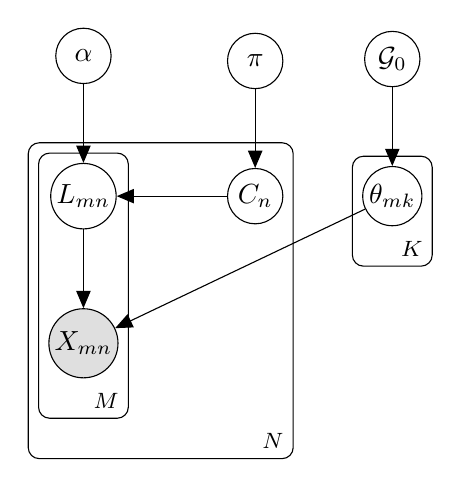
\begin{tikzpicture}

  % Define nodes
  \node[obs]                              (X) {$X_{mn}$};
  \node[latent, above=of X] 		(L) {$L_{mn}$};
  \node[latent, above=of L] 		(a) {$\alpha$};
  \node[latent, right=1.4cm of L]  (C) {$C_{n}$};
  \node[latent, above=of C] 		(p) {$\pi$};
  \node[latent, right=1cm of C]  (t) {$\theta_{mk}$};
  \node[latent, above=of t] 		(G) {$\mathcal{G}_{0}$};

  % Connect the nodes
  \edge {L,t} {X} ; %
  \edge {a,C} {L} ; %
  \edge {p} {C} ; %
  \edge {G} {t} ; %

  % Plates
  \plate {} {(t)} {$K$};
  \plate {yx} {(L)(X)} {$M$};
  \plate {} {(C)(X)(yx.north west)(yx.south west)} {$N$};

\end{tikzpicture}
%\endpgfgraphicnamed

%%% Local Variables: 
%%% mode: tex-pdf
%%% TeX-master: "example"
%%% End: 

	\emph{Graphical Model of BCC.}
  \end{center}
\end{minipage}
%\hfill
\begin{minipage}{0.4\textwidth}%\raggedright
  \begin{equation*}
  	\begin{aligned}
  		\mathbf{\pi} \; & \sim \; \mathcal{D}ir(\delta) \\
  		\alpha \; & \sim \; \mathcal{TB}(\mathit{a}, \beta, \frac{1}{K}) \\
  		\theta_{mk} \; & \sim \mathcal{G}_{0}(\cdot | \mathcal{H}) \\
  		C_{n} \mid \mathbf{\pi} \; & \sim \; \mathcal{C}at(\mathbf{\pi}) \\
  		L_{mn} \mid \alpha_{m}, C_{n} \; & \sim \; v(L_{mn}, C_{n}, \alpha_{m}) \\
  		X_{mn} \mid L_{mn}=k,\theta_{mk} \; & \sim \; f_{m}(\cdot | \theta_{mk}) 
  	\end{aligned} 
  \end{equation*} 
\end{minipage}
\vspace*{5mm}

\subsection{Bayesian inference for BCC model}\label{integr-bayes-inference-subsect}
The full joint distribution of the BCC model, by looking at the graphical representation factorizes as follows:
\begin{equation}%\scriptstyle
  \begin{aligned}
	P(\mathbb{X}, \mathbb{L}, \mathbb{C}, \pi , \Theta , \alpha) & = P(\mathbb{X}|\mathbb{L},\Theta) P(\mathbb{L}|\mathbb{C},\alpha) P(\mathbb{C}|\pi) P(\alpha) P(\pi) P(\Theta) \\
	  & = \bigg[\prod_{n}\bigg(\prod_{m} P(X_{mn}|L_{mn},\theta_{m,L_{mn}}) P(L_{mn}|C_{n},\alpha_{m})\bigg) P(C_{n}|\pi)\bigg] \\
	  & \; \quad \quad \quad \quad \quad \quad \quad \quad \quad \quad \quad \quad P(\alpha) P(\pi) \bigg(\prod_{m}\prod_{k} P(\theta_{mk})\bigg)
  \end{aligned}
\end{equation}
where the prior distribution $\mathcal{G}_{0}$ and the hyper-parameters ($\delta, \mathit{a}, \beta, \mathcal{H}$) are omitted for clarity.

To perform inference in the Bayesian framework, the posterior distribution of the variables needs to be estimated. By applying Bayes' theorem and conditioning on the observed data $\mathbb{X}$ from all data sources, the posterior distribution is the following:

\begin{equation}%\scriptstyle
	\begin{aligned}
	P(\mathbb{L},\mathbb{C},\pi,\Theta,\alpha | \mathbb{X}) & = \frac{P(\mathbb{X}|\mathbb{L},\mathbb{C},\pi,\Theta,\alpha) P(\mathbb{L},\mathbb{C},\pi,\Theta,\alpha)}{p(\mathbb{X})} \\
	& = \frac{P(\mathbb{X}|\mathbb{L},\Theta) P(\mathbb{L}|\mathbb{C},\alpha) P(\mathbb{C}|\pi) P(\alpha) P(\pi) P(\Theta)}{p(\mathbb{X})}
	\end{aligned}
\end{equation}
where we use the fact that $\mathbb{X}$ is conditionally independent of $\mathbb{C}, \pi$ and $\alpha$ given $\mathbb{L}$, \ie $\mathbb{X} \bigCI \mathbb{C}, \pi, \alpha \mid \mathbb{L}$, by looking at the \emph{Markov blanket} of $\mathbb{X}$. 

This posterior is intractable to compute, thus we need to resort to an approximation scheme. The algorithm that will be used is \emph{Gibbs sampling} \citep{Geman1984}. Deriving Gibbs sampling for this model requires deriving an expression for the \emph{full conditional} distribution of every random variable. From the graphical representation of the BCC model, we can infer the conditional independencies between the latent variables by looking at their \emph{Markov blanket}. 

For mathematical convenience, \emph{conjugate priors} should be used over the parameters, which would allow us to write analytically the full conditional distributions, and also draw samples from them. Thus:
\begin{itemize}
	\item $\pi_{k} \sim \mathcal{D}ir(\mathbf{\delta})$. For the mixing proportions a natural choice is a Dirichlet prior distribution, and the hyper-parameter vector $\mathbf{\delta}$ is set to $(1,...,1)$ so the prior is uniformly distributed in the $K-1$ simplex.
	\item $\alpha_{m} \sim \mathcal{TB}(\mathit{a}, \beta, \frac{1}{K})$. Which means that $\alpha_{m}$ follows a $Beta$ distribution with parameters $\mathit{a}, \beta$ truncated below by $\frac{1}{K}$.
	\item $\theta_{mk} \sim \mathcal{G}_{0}$. Where $\mathcal{G}_{0}$ is a conjugate prior distribution, so that sampling from the full conditional distribution $\mathcal{G}_{0}(\theta_{mk}|\mathbb{X}_{m}, \mathbb{L}_{m})$ is feasible.
\end{itemize}

\noindent\textbf{Gibbs sampling algorithm for BCC}: 
\begin{itemize}
\item {Initially, at simulation step 0, parameter values are chosen arbitrarily.}
\item {Suppose at simulation step $\tau$ we have sampled values $\mathbb{L}^{(\tau)}, \Theta^{(\tau)}, \alpha^{(\tau)}, \mathbb{C}^{(\tau)}, \pi^{(\tau)}$.}
\item { At simulation step $\tau + 1$, the Gibbs sampler continues as follows:
\begin{equation*}%\scriptstyle
  \begin{aligned}
    L_{mn}^{(\tau+1)} \mid X_{mn}, \Theta_{m}^{(\tau)}, C_{n}^{(\tau)}, \alpha_{m}^{(\tau)} & \sim v(L_{mn}, C_{n}, \alpha_{m}) f_{m}(X_{mn}|\theta_{mk}) \\
	\theta_{mk}^{(\tau+1)} \mid \mathbb{L}_{m}^{(\tau+1)}, \mathbb{X}_{m} & \sim \mathcal{G}_{0}(\theta_{mk} \mid \mathbb{X}_{m}, \mathbb{L}_{m} = k; \mathcal{H}) \\
%	\alpha_{m}^{(\tau+1)} \mid \mathbb{L}_{m}^{(\tau+1)}, \mathbb{C}^{(\tau)} & \sim \mathcal{TB} \big(\mathit{a}+\sum_{n}\mathbbm{1}(L_{mn}=k,C_{n}=k), \\
%	  & \quad \quad \quad \; \beta + N -\sum_{n}\mathbbm{1}(L_{mn}=k,C_{n}=k), \frac{1}{K}\big) \\
	\alpha_{m}^{(\tau+1)} \mid \mathbb{L}_{m}^{(\tau+1)}, \mathbb{C}^{(\tau)} & \sim \mathcal{TB} \big(\mathit{a} + Q_{mk}, \beta + N - Q_{mk}, \frac{1}{K}\big) \\
	C_{n}^{(\tau+1)} \mid L_{mn}^{(\tau+1)}, \alpha^{(\tau+1)}, \pi^{(\tau)} & \sim \pi_{k} \prod_{m}v(L_{mn}, C_{n}, \alpha_{m}) \\
	\pi_{k}^{(\tau+1)} \mid \mathbb{C}^{(\tau+1)} & \sim \mathcal{D}ir\big(\delta + \sum_{n}\mathbbm{1}(C_{n}=k)\big)
  \end{aligned}
\end{equation*}
where $Q_{mk} = \sum_{n}\mathbbm{1}(L_{mn}=k,C_{n}=k)$, and $\mathbbm{1}(\cdot,\cdot)$ is the indicator function, equal to 1 if the quantities inside the function are satisfied, and 0 otherwise.
}
\end{itemize}

\subsection{Extending BCC model for NGS data}\label{integr-extension-subsect}
As it was aforementioned, with the advent of high-throughput sequencing methods, BCC needs to be extended so it can model data that follow different probability distributions.

Due to conditional independence structure of the mixture models, changing the observation model for data source $\mathbb{X}_{m}$ does not affect the mixing proportions $\pi$, the adherence parameter $\alpha$, and the overall clustering assignments $\mathbb{C}$. Thus, modelling and subsequently inferring these variables remains the same as it was explained in the previous section.

The source-specific clustering assignments $\mathbb{L}_{m}$ depend on the observation model of the data sources $\mathbb{X}_{m}$. Hopefully, the update equations for $\mathbb{L}_{m}$ on each Gibbs simulation step are straightforward to adapt, since we just need to evaluate $f_{m}(X_{mn}|\theta_{m})$ pointwise, which for most known probability distribution is easy to compute.

Thus, the focus of this section is mainly in modelling, \ie defining a prior distribution, and inferring the parameters $\theta_{m}$ of the observation model. 

\subsubsection*{Gaussian observation model}
For completeness we provide details for the Gaussian observation model, as it was described in \citet{Lock2013}. When the data source $\mathbb{X}_{m}$ follows a Gaussian mixture distribution, we have:
\begin{equation}
	X_{mn} \mid L_{mn} = k, \theta_{mk} \sim \mathcal{N}\big(\mu_{mk}, \tau_{mk}^{-1}\big)
\end{equation}
where $\mathcal{N}$ denotes the \emph{Normal} or \emph{Gaussian} distribution, $\mu_{mk}$ is the \emph{mean} parameter, and $\tau_{mk}$ is the \emph{precision} parameter, \ie the reciprocal of the variance, $\tau_{mk} = \frac{1}{\sigma_{mk}^{2}}$.

We choose a \emph{Normal-Gamma} conjugate prior distribution for the parameters $\theta_{mk} = (\mu_{mk}, \tau_{mk})$, that is:
\begin{equation}
	\theta_{mk} \sim \mathcal{NG}amma\big(\mu_{m0}, \tau_{m0}, \mathit{a}_{m0}, \beta_{m0}\big)
\end{equation}
where hyper-parameters $\mu_{m0}, \tau_{m0}$ are the same as defined above, and $\mathit{a}_{m0}, \beta_{m0}$ are the \emph{shape} and \emph{rate} hyper-parameters of the \emph{Gamma} distribution, respectively.

Thus, on each iteration step of Gibbs algorithm, we have the following updates for each parameter:
\begin{equation}
  \begin{aligned}
  	\tau_{mk} \mid \mathbb{L}_{m}=k, \mathbb{X}_{m} \;& \sim \;\mathcal{G}amma\big(\hat{\mathit{a}}_{m0}, \hat{\beta}_{m0}\big) \\
	\mu_{mk} \mid \tau_{mk}, \mathbb{L}_{m}=k, \mathbb{X}_{m} \; & \sim \; \mathcal{N}\big(\hat{\mu}_{m0}, (\hat{\tau}_{m0} \tau_{mk})^{-1}\big)
  \end{aligned}
\end{equation}
The posterior parameter values for the $\mathcal{NG}(\cdot,\cdot,\cdot,\cdot)$ distribution are calculated as follows:
\begin{equation}
  \begin{aligned}
  	\hat{\mu}_{m0} \; &= \; \frac{\tau_{m0}\mu_{m0} + N_{mk}\mathcal{X}_{mk}}{\tau_{m0} + N_{mk}}\\
  	\hat{\tau}_{m0} \; &= \; \tau_{m0} + N_{mk}\\
  	\hat{\mathit{a}}_{m0} \; &= \; \mathit{a}_{m0} + \frac{N_{mk}}{2}\\
  	\hat{\beta}_{m0} \; &= \; \beta_{m0} + \frac{SSD_{mk}}{2} + \frac{N_{mk}\tau_{m0}(\mathcal{X}_{mk} - \mu_{m0})}{2(N_{mk}+\tau_{m0})}
  \end{aligned}
\end{equation}
where: 
\begin{equation}
  \begin{aligned}
		N_{mk} \; &= \; \sum_{n}\mathbbm{1}(L_{mn}=k)\\ 
		\mathcal{X}_{mk} \; &= \; \frac{\sum_{n}\mathbbm{1}(L_{mn}=k)X_{mn}}{N_{mk}} \\
		SSD_{mk} \; &= \; \sum_{n}\mathbbm{1}(L_{mn}=k)(X_{mn}-\mathcal{X}_{mk})^{2}
  \end{aligned}
\end{equation} 

If the data source $\mathbb{X}_{m}$ is $D_{m}$-dimensional, then we can use either a $D_{m}$ dimensional \emph{Normal-Gamma} prior, if we assume a $D_{m} \times D_{m}$ \emph{diagonal precision} matrix, or a \emph{Normal-Wishart} prior, if we assume a $D_{m} \times D_{m}$ \emph{full precision} matrix \cite[Ch. 2]{Bishop2006}.

\subsubsection*{Binomial observation model}
When the data source $\mathbb{X}_{m}$ follows a Binomial mixture distribution, we have:
\begin{equation}
	X_{mn} \mid L_{mn} = k, \theta_{mk} \sim \mathcal{B}inom\big(t_{mk}, \rho_{mk}\big)
\end{equation}
where $t_{mk}$ is \emph{known} and denotes the total number of experiments, and $\rho_{mk}$ is the parameter for the probability of success.

We choose a \emph{Beta} conjugate prior distribution for the parameter $\rho_{mk}$, that is:
\begin{equation}
	\rho_{mk} \sim \mathcal{B}eta\big(\mathit{a}_{m0}, \beta_{m0}\big)
\end{equation}
where $\mathit{a}_{m0}$ and $\beta_{m0}$ are the \emph{shape} hyper-parameters of the \emph{Beta} distribution.

Thus, on each iteration step of Gibbs algorithm, we have the following update for the $\rho_{mk}$ parameter:
\begin{equation}
  \begin{aligned}
  	\rho_{mk} \mid \mathbb{L}_{m}=k, \mathbb{X}_{m} \;& \sim \;\mathcal{B}eta\big(\hat{\mathit{a}}_{m0}, \hat{\beta}_{m0}\big) \\
  \end{aligned}
\end{equation}
where the posterior parameter values for the $\mathcal{B}eta(\cdot,\cdot)$ distribution are calculated as follows:
\begin{equation}
  \begin{aligned}
  	\hat{\mathit{a}}_{m0} \; &= \; \mathit{a}_{m0} + \sum_{n}\mathbbm{1}(L_{mn}=k)X_{mn} \\
  	\hat{\beta}_{m0} \; &= \; \beta_{m0} +  \sum_{n}\mathbbm{1}(L_{mn}=k)(r_{mn} - X_{mn})
  \end{aligned}
\end{equation}

\subsubsection*{Poisson observation model}
When the data source $\mathbb{X}_{m}$ follows a Poisson mixture distribution, we have:
\begin{equation}
	X_{mn} \mid L_{mn} = k, \theta_{mk} \sim \mathcal{P}ois\big(\lambda_{mk}\big)
\end{equation}
where $\lambda_{mk}$ denotes the mean and variance parameter.

We choose a \emph{Gamma} conjugate prior distribution for the parameter $\lambda_{mk}$, that is:
\begin{equation}
	\lambda_{mk} \sim \mathcal{G}amma\big(\mathit{a}_{m0}, \beta_{m0}\big)
\end{equation}
where $\mathit{a}_{m0}$ and $\beta_{m0}$ are the \emph{shape} and \emph{rate} hyper-parameters of the \emph{Gamma} distribution.

Thus, on each iteration step of Gibbs algorithm, we have the following update for the $\lambda_{mk}$ parameter:
\begin{equation}
  \begin{aligned}
  	\lambda_{mk} \mid \mathbb{L}_{m}=k, \mathbb{X}_{m} \;& \sim \;\mathcal{G}amma\big(\hat{\mathit{a}}_{m0}, \hat{\beta}_{m0}\big) \\
  \end{aligned}
\end{equation}
where the posterior parameter values for the $\mathcal{G}amma(\cdot,\cdot)$ distribution are calculated as follows:
\begin{equation}
  \begin{aligned}
  	\hat{\mathit{a}}_{m0} \; &= \; \mathit{a}_{m0} + \sum_{n}\mathbbm{1}(L_{mn}=k)X_{mn} \\
  	\hat{\beta}_{m0} \; &= \; \beta_{m0} +  \sum_{n}\mathbbm{1}(L_{mn}=k)
  \end{aligned}
\end{equation}

\section{Synthetic Experiments} \label{integr-synth-exper-sect}
In this section we present some experiments based on synthetic data that illustrate certain features of the BCC model. Initially, we will describe how the synthetic data were generated. Then, we will experiment with these data to evaluate the accuracy of the model in estimating the adherence parameter $\alpha$, but also the clustering accuracy. Finally, the mixing of the chains and convergence diagnostics of the MCMC simulations will be demonstrated.

\subsection{Generating Synthetic Datasets} \label{integr-synth-data-sect}
As it is aforementioned, the mixture model is a \emph{generative model}, thus, it gives us information for generating data. To generate data $X_{mn}$, we start with the parameters that are in the highest levels of the graphical model, since they are independent. Then, we move down in lower levels and generate samples conditioning on the values of their \emph{parents}, \ie the parameters that are in the higher levels. 

For our synthetic dataset, we assume that we have $M=3$ one-dimensional data sources, and each data source consists of $N=1000$ objects, \ie $\mathbb{X}_{m} : 1 \times 1000$. Each data source has a different observation model, that is we have:
\begin{equation*}
  \begin{aligned}
  	\mathbb{X}_{1} \; & \sim \; \mathcal{N}(\mu, \tau) \\
  	\mathbb{X}_{2} \; & \sim \; \mathcal{B}inom(r, \rho) \\
  	\mathbb{X}_{3} \; & \sim \; \mathcal{P}ois(\lambda)
  \end{aligned}
\end{equation*}
Finally, we assume that there are $K=2$ clusters on each data source, hence, the overall clustering assignments $\mathbb{C}$ are divided in $C_{n}=1$ for $n \in \lbrace 1,...,500 \rbrace$, and $C_{n}=2$ for $n \in \lbrace 501,...,1000 \rbrace$. 

The procedure for generating the synthetic datasets proceeds as follows:
\begin{enumerate}
	\item{
		Sample $\alpha$ from $\mathcal{U}niform(\frac{1}{K}, 1)$ distribution. We assume that we have equal adherence for each data source, that is, $\alpha_{1} = \alpha_{2}$
	}
	\item{
		Generate the source-specific clusterings $L_{mn} \in \lbrace 1,2 \rbrace$ with probabilities $p(L_{mn} = C_{n}) = \alpha$ and $p(L_{mn} \neq C_{n}) = 1 - \alpha$
	}
	\item{
		Generate data $X_{mn}$ as follows:
		\begin{itemize}
			\item{
				\textbf{m=1}: If $L_{mn}=1 : X_{mn} \sim \mathcal{N}(1.5, 1)$. If $L_{mn}=2 : X_{mn} \sim \mathcal{N}(-1.5, 1)$
			}
			\item{ 
				\textbf{m=2}: If $L_{mn}=1 : X_{mn} \sim \mathcal{B}inom(50, .2)$. If $L_{mn}=2 : X_{mn} \sim \mathcal{B}inom(50, .7)$
			}
			\item{ 
				\textbf{m=3}: If $L_{mn}=1 : X_{mn} \sim \mathcal{P}ois(8)$. If $L_{mn}=2 : X_{mn} \sim \mathcal{P}ois(15)$
			}
		\end{itemize}	
	}
\end{enumerate}

We generated 100 synthetic datasets following the procedure described above, and for each realization the model parameters were estimated using BCC. For the adherence parameter a $\mathcal{TB}(1, 1, \frac{1}{K})$ prior was introduced. All the parameters of the different observation models and the mixing proportions were initialized using \emph{k-means} algorithm \citep{MacQueen1967}. Finally, the total number of MCMC iterations was set to $T=10,000$, and the first $2,000$ iterations were discarded (\ie burn-in period). 
\subsection{Adherence Parameter Accuracy } \label{integr-synth-alpha-sect}
In this experiment, we test if the BCC model can recover the value of the adherence parameter with reasonable accuracy. Since, we have the ground truth values for $\alpha$ from the synthetic data, we can compare them with the estimated $\hat{\alpha}$ returned from the BCC model. \emph{Fig. \ref{adherence-test-pic}} depicts the estimated $\hat{\alpha}$ (on the y-axis) versus the true $\alpha$ (on the x-axis) for the 100 realizations of the synthetic data. For each realization, we show the \emph{mean} value of the estimated $\hat{\alpha}$ together with its $95$\% \emph{credible interval} based on the $2.5 - 97.5$ percentiles of the MCMC simulations. 
\begin{figure}[!ht]
\begin{center}
 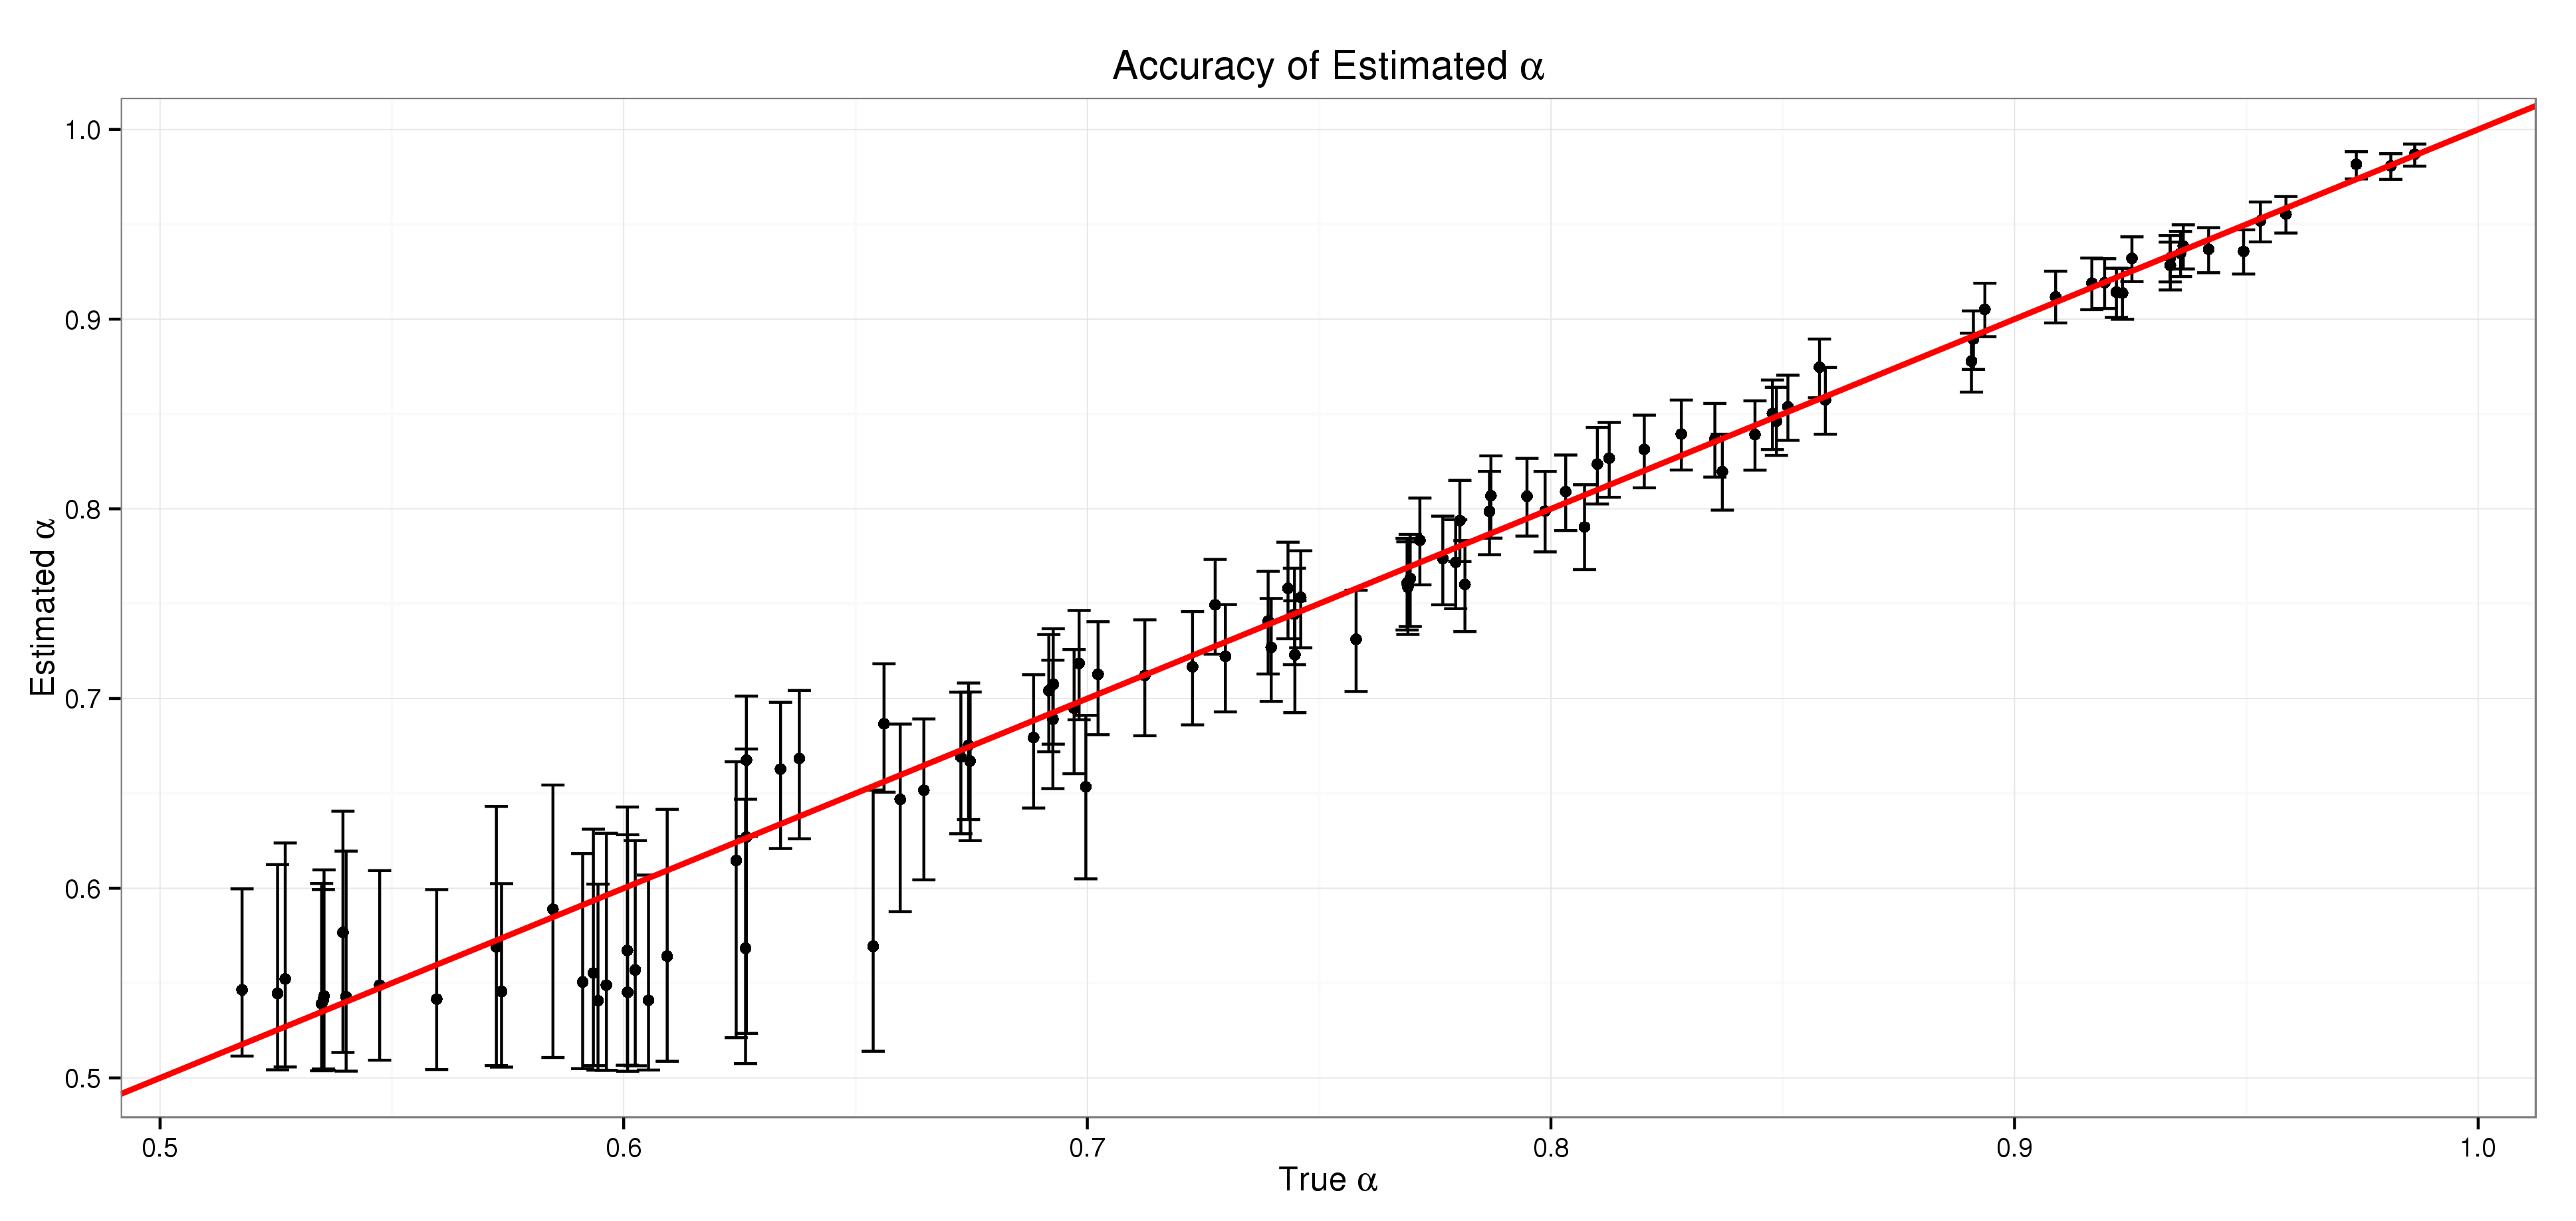
\includegraphics[scale = 0.41]{images/adherenceTest.png}
\caption{\emph{Comparison of estimated $\hat{\alpha}$ (y-axis) versus true $\alpha$ (x-axis) for the 100 realizations of the synthetic data. Values in the main diagonal show perfect agreement. For each realization, the mean value of $\hat{\alpha}$ and the $95$\% credible interval is shown.}}
\label{adherence-test-pic}
\end{center}
\end{figure}

In general, we observe that the true value of $\alpha$ can be recovered with reasonable accuracy, and more specifically in 97 of 100 realizations the $95$\% credible interval contains the true value of $\alpha$. Finally, it should be noted that as $\alpha$ increases, the estimate uncertainty decreases (\ie $95$\% credible interval shrinks), thus the BCC model becomes more accurate. This ... is expected, if we think the role of the adherence parameter, and has the following explanation. 

When $\alpha \approx 1$, it means that there is a perfect agreement between the source-specific and the overall clustering assignments. This implies, that there are clear associations between the data sources, thus we would be able to combine them together without losing predictive power. Intuitively, the problem reduces to performing a single 'joint' clustering which is an easier task, especially for our experiments, where the different clusters are well separated. On the other extreme, when $\alpha \approx 0.5$, there is no agreement and any association between the data sources could be random. This is similar to performing a separate clustering on each data source followed by post-hoc integration, but since there are no common features between the data sources, overall clustering assignments could be due to chance, that is why the model has higher variability and also makes less accurate predictions. 
\subsection{Clustering Accuracy} \label{integr-synth-cluster-sect}
Evaluation of the \emph{clustering accuracy} for the BCC model, will be made on the same 100 realizations of the synthetic data that were used for evaluating the accuracy of the adherence parameter.

The metrics considered are the source-specific and overall clustering errors, $\mathbf{L}_{error}$ and $\mathbf{C}_{error}$ respectively, which compute the average number of incorrect cluster assignments. 
\begin{equation}
  \begin{aligned}
  	\mathbf{L}_{error} & = \frac{\sum\limits_{m=1}^{M}\sum\limits_{n=1}^{N}\mathbbm{1}(\hat{L}_{mn} \neq L_{mn})}{MN} \\
  	\mathbf{C}_{error} & = \frac{\sum\limits_{n=1}^{n}\mathbbm{1}(\hat{C}_{n} \neq C_{n})}{N}
  \end{aligned}
\end{equation}
where $\hat{L}_{mn}, \hat{C}_{n}$ denote the estimated source-specific and overall clustering assignments, and $\mathbbm{1}(\cdot)$ is the indicator function.

The relative error for the overall and the source-specific clusterings is shown in \emph{Fig. \ref{source-error-pic}} and \emph{Fig. \ref{overall-error-pic}}, respectively. The results in each figure are shown as a function of $\alpha$. \emph{LOESS} regression \citep{Cleveland1979} is fit to the results so as to produce smooth curves. 

Care should be taken when comparing the results between the two figures, since the y-axis limits for $\mathbf{L}_{error}$ are $(0,0.12)$, whereas for $\mathbf{C}_{error}$ are $(0,0.52)$. This difference is not surprising, since the clustering problem is much easier when performed on each data source individually, especially for our synthetic data, where the different clusters are well separated. 

Both, $\mathbf{L}_{error}$ and $\mathbf{C}_{error}$ decrease as the value of $\alpha$ increases, and they almost reach 0, when $\alpha \approx 1$. Both of these results confirm, in a different view, the results shown in \emph{Fig. \ref{adherence-test-pic}}, since the lower the error, the more accurate the estimates for the value of $\alpha$.

\citet{Lock2013} conducted further analysis on the clustering accuracy by comparing the BCC model with separate clustering, joint clustering and dependent clustering, where they showed that BCC can be seen as a flexible bridge between the extremes of separate and joint clusterings.

\begin{figure}[!ht]
\begin{center}
 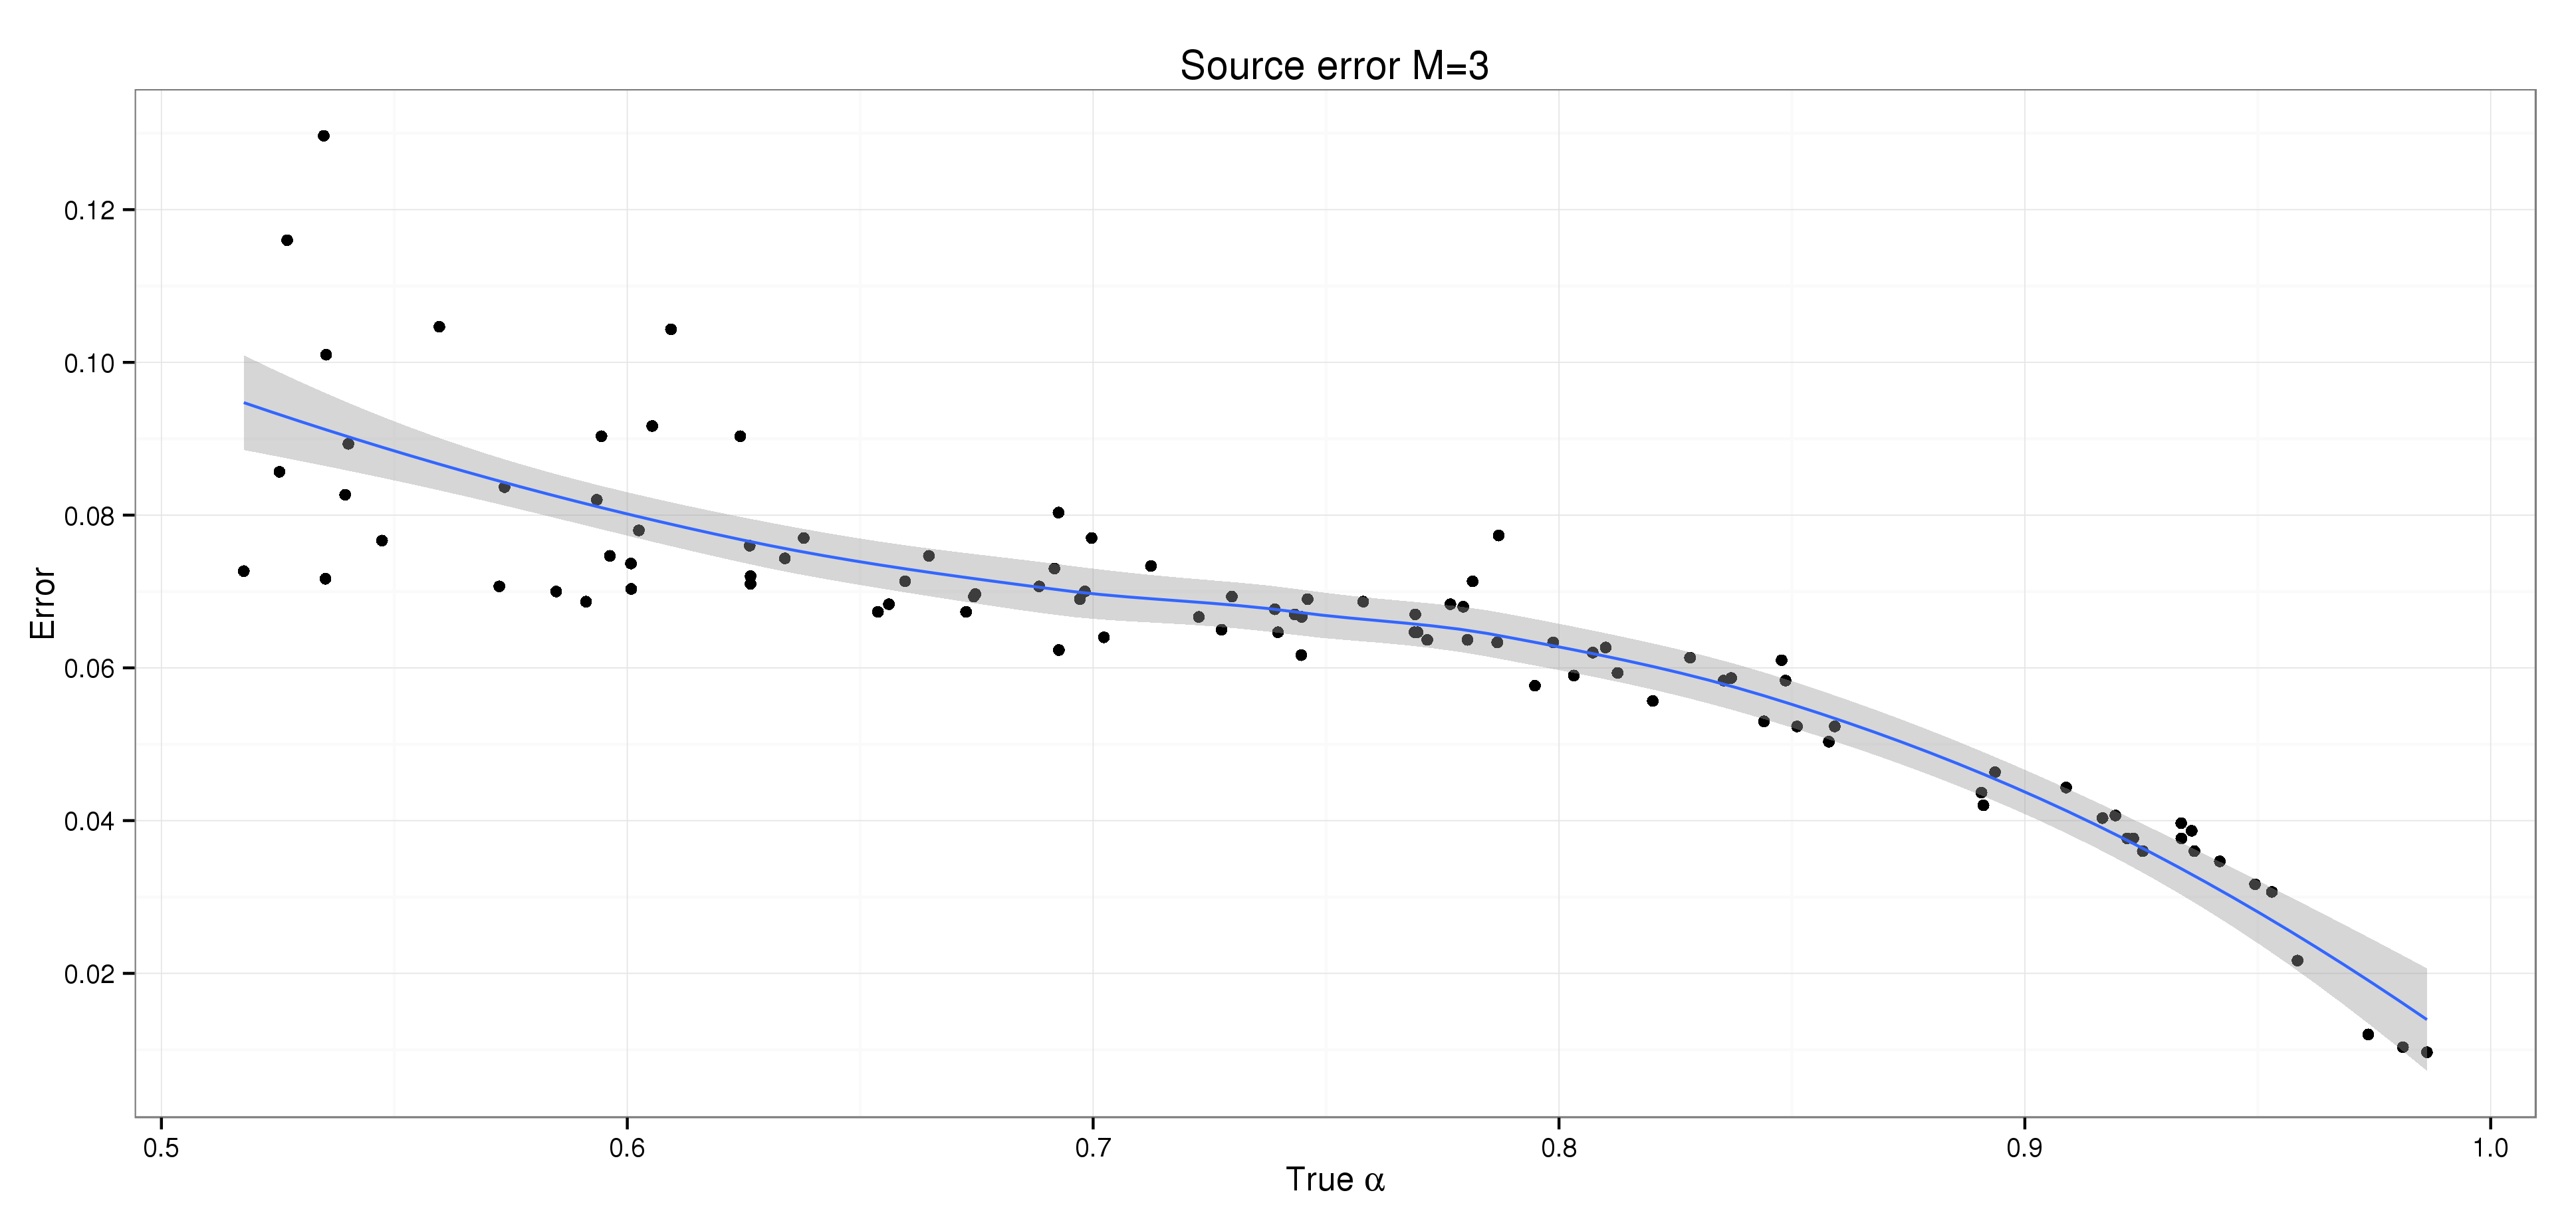
\includegraphics[scale = 0.41]{images/sourceError.png}
\caption{\emph{Source-specific clustering error as a function of $\alpha$ for 100 realizations with $M=3$ data sources and $K=2$ clusters.}}
\label{source-error-pic}
\end{center}
\end{figure}
\begin{figure}[!ht]
\begin{center}
 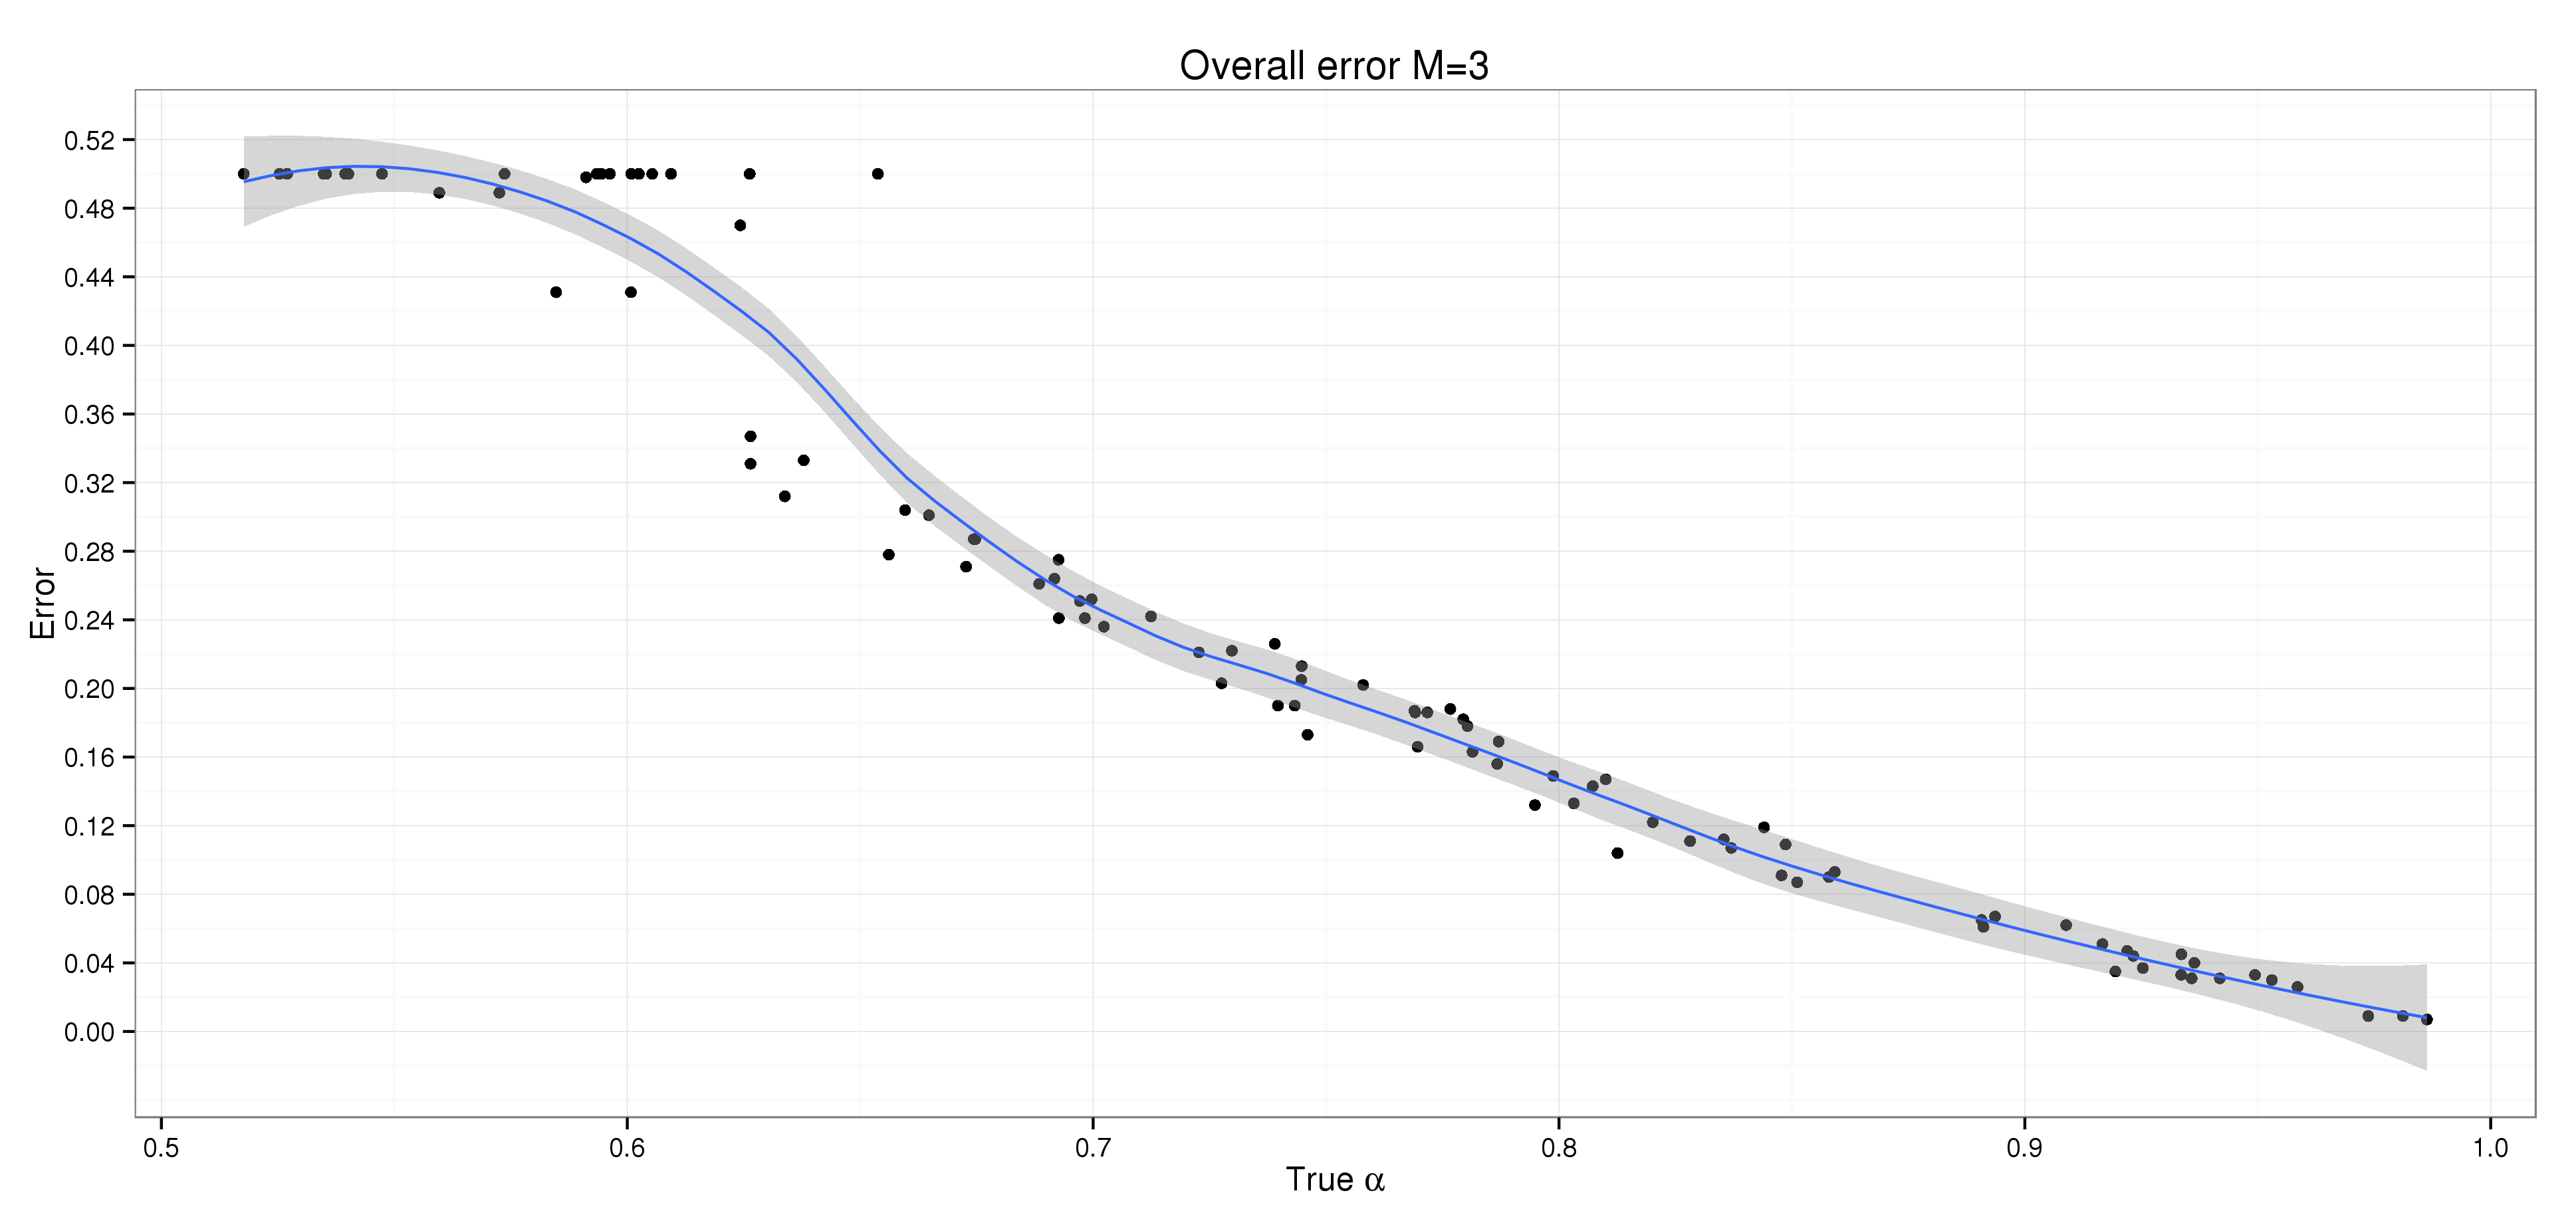
\includegraphics[scale = 0.41]{images/overallError.png}
\caption{\emph{Overral clustering error as a function of $\alpha$ for 100 realizations with $M=3$ data sources and $K=2$ clusters.}}
\label{overall-error-pic}
\end{center}
\end{figure}
\subsection{MCMC Chain Analysis} \label{integr-synth-chain-sect}
For the analysis of the MCMC simulations, one realization of the synthetic data is chosen randomly, and the CODA package \citep{Plummer2006} is used. 

The main question to ask when monitoring an MCMC chain, is when to stop the MCMC algorithm, that is to assess when the chain has converged to the \emph{stationary} distribution. Unfortunately, there are no clear convergence markers, or theoretical guarantees to tell us when to stop the MCMC algorithm, thus, the choice is mostly empirical by using certain techniques for convergence diagnoses.

A less ambitious goal is to experimentally assess the \emph{mixing} of the chain, \ie how well the MCMC samples explore the support of the posterior distribution, and also the degree of correlation between successive random samples. Ideally, at each iteration step the samples should be \emph{independent} in order to perform Monte Carlo integration with few samples. But, MCMC samples are slightly dependent, thus the MCMC algorithm converges slowly to the target distribution; however, when the correlation between successive samples is small, the algorithm explores faster the posterior space, hence it converges faster.

\emph{Fig. \ref{trace-density-l-pic}} shows the output of the simulated chain across MCMC iterations, for the $\lambda_{k}$ parameters of the Poisson mixture model. On the left side we have the \emph{trace plots}, which show the values that the parameters took at each MCMC iteration. On the right side we have the \emph{marginal density} plot for each parameter, which is a non-parametric estimate of the distribution of the parameters in the chain. The traces have 8000 iterations, since the first 2000 iterations are discarded, \ie burn-in period.
\begin{figure}[!ht]
\begin{center}
 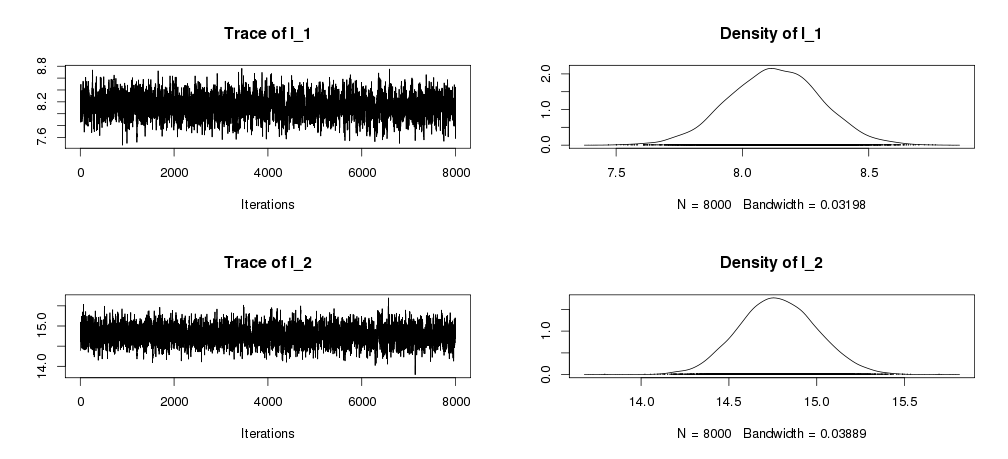
\includegraphics[scale = 0.40]{images/traceDensityL.png}
\caption{\emph{\textbf{Left:} Trace-plots for the $\lambda_{k}$ parameters of the Poisson mixture. \textbf{Right:} Corresponding marginal density plots.}}
\label{trace-density-l-pic}
\end{center}
\end{figure}

From the traces it is clear that the mixing of the chain is good, and the algorithm has found two modes of the posterior distribution where each parameter individually explores. Parameter $\lambda_{1}$ explores values around 8, whereas $\lambda_{2}$ explores values around 15, which are the true values of the generated Poisson mixtures, as explained in \emph{Section \ref{integr-synth-data-sect}}. Since, each parameter moves over a range of values around its mode and does not \emph{jump} across different modes, the marginal density plots are \emph{unimodal}.

To assess correlation between successive samples, the \emph{Auto Correlation Function (ACF)} is used. ACF measures the correlation of the values of the chain at different points in time. The \emph{lag} is the time-distance between the pair of values to be compared. The ACF for the $\lambda_{k}$ parameters of the Poisson mixture model is shown in \emph{Fig. \ref{acfL-pic}}. It is evident that the samples become uncorrelated quite fast, when $lag \approx 10$, and this allows the chain to mix well.
\begin{figure}[!ht]
\begin{center}
 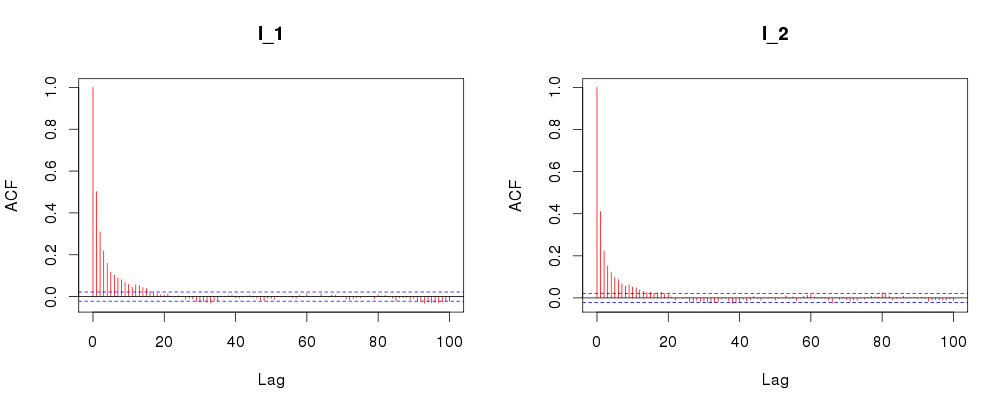
\includegraphics[scale = 0.40]{images/acfL.png}
\caption{\emph{Auto Correlation Function for the $\lambda_{k}$ parameters of the Poisson mixture. The maximum lag is set to 100.}}
\label{acfL-pic}
\end{center}
\end{figure}

The major approach for monitoring and assessing convergence of the MCMC simulation to the stationary distribution is to use multiple chains simultaneously, and then perform a statistical diagnostic test on the chains. The most widely used method is the Gelman-Rubin diagnostic \citep{Gelman1992, Brooks1997}. Basically, the method is based in analysing multiple MCMC chains by measuring whether there is a significant difference between the variance within each chain and the variance between the multiple chains. The assumption is that at convergence, the chains will have mixed well, thus the distributions of the MCMC simulations for the within and between chain variances will be very similar. Thus, we would expect that the ratio of these quantities would be around 1. The square root of this ratio is called the \emph{potential scale reduction factor (PSRF)}. 

When assessing convergence using the Gelman-Rubin diagnostic, PSRF should be close to 1 to denote chain convergence, otherwise the chain has either not reached yet the stationary distribution, or the posterior is multi-modal and different chains may converge to different local modes. A rule of thumb, if to choose really dispersed initial values between the different chains, so the MCMC chains can explore different parts of the posterior distribution as they converge to the stationary distribution.

The Gelman-Rubin diagnostic was used to assess the convergence of the $\lambda_{k}$ parameters of the Poisson mixture model, using three different MCMC chains. \emph{Fig. \ref{psrf-lambda-pic}} shows how the PSRF (or shrink factor) evolves over time. In the first few thousand iterations the shrink factor is not stable (\ie there are small bumps), but then it seems to converge, and the $PSRF \approx 1$.  
\begin{figure}[!ht]
\begin{center}
 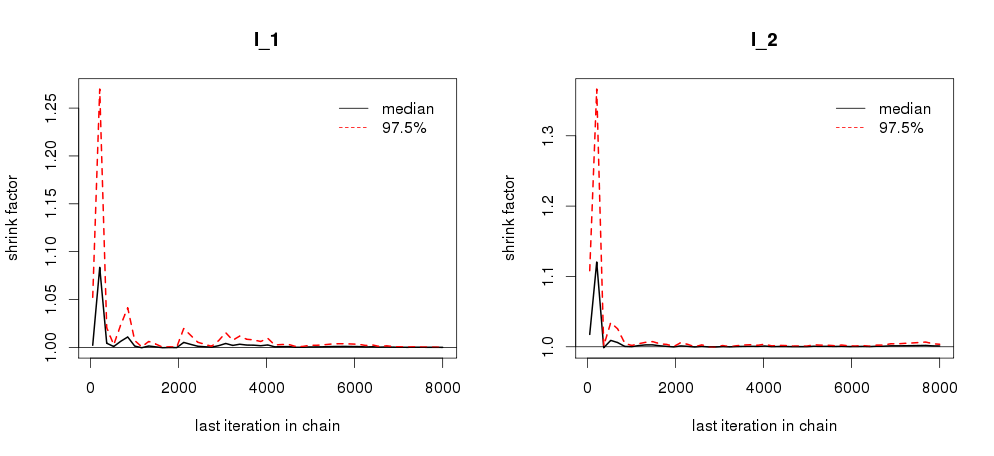
\includegraphics[scale = 0.41]{images/psrf-l.png}
\caption{\emph{Convergence of the MCMC simulations for the $\lambda_{k}$ parameters of the Poisson mixture, using the Gelman-Rubin diagnostic.}}
\label{psrf-lambda-pic}
\end{center}
\end{figure}

For brevity, only the $\lambda_{k}$ parameters of the Poisson mixture model were shown for analysis of convergence of the MCMC simulations, but similar results were obtained also for all the other parameters inferred from the BCC model. Also, the different convergence diagnostics methods were introduced without in-depth discussion. A comprehensive discussion on the convergence diagnostics for MCMC chains, including many examples, are provided in \citep{Brooks1999, Robert2009}.
\subsection{Label-switching problem} \label{integr-synth-label-sect}
This section concerns the \emph{label switching} problem that often arises when performing a Bayesian analysis on mixture models, as it was explained in \emph{Section \ref{fdmm-relable-subsect}}.

To illustrate the problem, a different synthetic dataset is used, consisting of $M=3$ data sources, where each data source is generated from $K=3$ well separated clusters. 

\emph{Fig. \ref{labelBP-pic}} shows the output of the simulated chain across MCMC iterations, for the $\rho_{k}$ parameters of the Binomial mixture model. Label switching is evident in the trace plot on the left side of the figure. More specifically, $\rho_{1}$ and $\rho_{2}$ parameters switch labels across different times in the chain, resulting in a bimodal marginal density plot for each parameter, whereas $\rho_{3}$ is concentrated on a different mode and explores the region around that posterior mode. 
\begin{figure}[!ht]
\begin{center}
 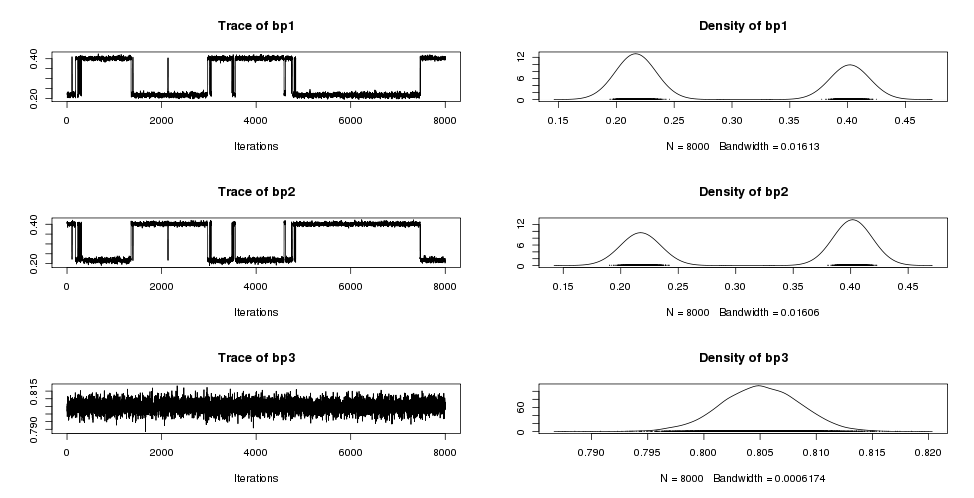
\includegraphics[scale = 0.39]{images/labelBP.png}
\caption{\emph{Trace plots and corresponding marginal density plots for the $\rho_{k}$ parameters of the Binomial mixture. Label-switching is evident for $\rho_{1}$ and $\rho_{2}$ parameters.}}
\label{labelBP-pic}
\end{center}
\end{figure}

Estimating quantities of interest, \eg posterior mean, from the marginal distributions of $\rho_{1}$ and $\rho_{2}$ parameters, would lead to nonsensical answers. The approach we took for solving this problem is \citet{Stephens2000} relabelling algorithm, which tries to permute the hidden labels of the MCMC output in such a way that the marginal posterior of each parameter is, as far as possible, unimodal. The \emph{label.switching} package of \citet{Papastamoulis2015} is used for running \emph{Stephens} algorithm. 

The outcome of the algorithm is shown in \emph{Fig. \ref{labelBP-stephens-pic}}. Even though label switching is not completely vanished, the posterior marginal densities of each parameter have become unimodal, hence we can compute quantities of interest.
\begin{figure}[!ht]
\begin{center}
 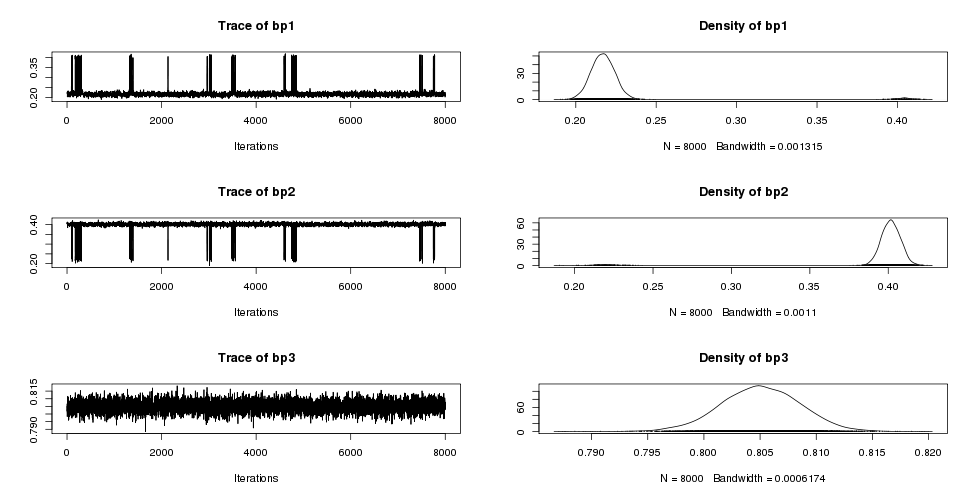
\includegraphics[scale = 0.39]{images/labelBP-stephens.png}
\caption{\emph{Trace plots and corresponding marginal density plots for the $\rho_{k}$ parameters of the Binomial mixture, after running the \citet{Stephens2000} relabelling algorithm.}}
\label{labelBP-stephens-pic}
\end{center}
\end{figure}

%\chapter{Discussion} \label{discussion-chapter}

%\section{Introduction} \label{data-intro-sect}
This chapter is concerned with introducing data generated from Next Generation Sequencing (NGS) technology, also termed as high-throughput sequencing. \emph{DNA sequencing} is the process of determining the complete order of DNA nucleotides of an organism's genome at a single time. Until recently, the method of choice for DNA sequencing was the \emph{chain termination} method developed by \citet{Sanger1977}. This technology, and its variants, even though they were widely adopted, they had inherent limitations in throughput, scalability, speed and cost. 

NGS technology \citep{Shendure2008, Mardis2008}, performs massively parallel sequencing on DNA fragments, producing thousands or millions of DNA fragment sequences, called \emph{reads}, concurrently. This yields substantially higher throughput and allows for entire genomes to be sequenced within a day. By reducing the cost by over two orders of magnitude from traditional Sanger sequencing methods \citep{Shendure2008}, DNA sequencing became accessible for smaller labs, allowing for rapid development of applications in fields related to biological and biomedical sciences. Even though, millions of biological data are generated from NGS technology, computational data analysis is still a challenging task.


%%%%%%%%
%% Any appendices should go here. The appendix files should look just like the
%% chapter files.
\appendix
\chapter{Partial derivatives for M-step} \label{derivatives-m-step-s}

We need to compute the partial derivatives w.r.t. parameters $\theta_{k}$ of the following quantity:
\begin{equation} \label{parameters-est2-EM-f-app}
  \begin{split}
	\ell(\theta_{k}) & \triangleq \sum_{i} \sum_{k} \gamma(z_{ik}) \log p(\mathbf{y}_{i}|\mathbf{f}_{i}, \theta_{k}) \\
					 & = \sum_{i} \sum_{k} \gamma(z_{ik}) \sum_{l} \log \bigg(Binom \big(t_{il}, \Phi(g_{il}; \theta_{k})\big) \bigg) \\
					 & \propto  \sum_{i} \sum_{k} \gamma(z_{ik}) \sum_{l} \bigg(m_{il} \log \Phi(g_{il}; \theta_{k}) + \big(t_{il} - m_{il} \big) \log \big(1 - \Phi(g_{il}; \theta_{k})\big)\bigg)
  \end{split}
\end{equation}
where $\theta_{k} = (\alpha, \beta, c)$ in the example of $2^{nd}$ degree polynomial, i.e. $g_{il} = \alpha x^{2} + \beta x + c$. To not clutter notation, let $\Phi(g_{il}) = \Phi(g_{il}; \theta_{k})$. Thus, for the partial derivatives w.r.t. $\alpha$ parameter we have the following derivation:

\begin{equation} \label{derivative-a-f-app}
  \begin{split}
	\frac{\partial \ell(\theta_{k})}{\partial \alpha} & = \sum_{i} \gamma(z_{ik}) \sum_{l} \bigg[ m \frac{\partial}{\partial \alpha}\big(\log \Phi(g_{il})\big) + (t-m) \frac{\partial}{\partial \alpha}\big(\log \big[1 - \Phi(g_{il})\big]\big)\bigg] \\
		& = \sum_{i} \gamma(z_{ik}) \sum_{l} \bigg[ \frac{m}{\Phi(g_{il})} \frac{\partial \Phi(g_{il})}{\partial g_{il}} \frac{\partial g_{il}}{\partial \alpha} + \frac{t - m}{1 - \Phi(g_{il})}\bigg( -\frac{\partial \Phi(g_{il})}{\partial g_{il}} \frac{\partial g_{il}}{\partial \alpha} \bigg) \bigg] \\
		& = \sum_{i} \gamma(z_{ik}) \sum_{l} \bigg[ \frac{m}{\Phi(g_{il})} x_{il}^{2} \mathbf{\phi}(g_{il}) - \frac{t - m}{1 - \Phi(g_{il})} x_{il}^{2} \mathbf{\phi}(g_{il}) \bigg]\\
		& = \sum_{i}  \gamma(z_{ik}) \sum_{l} \bigg[ x_{il}^{2} \mathbf{\phi}(g_{il})\bigg(\frac{m}{\Phi(g_{il})} - \frac{t - m}{1 - \Phi(g_{il})}\bigg) \bigg] \\
		& = \sum_{i}  \gamma(z_{ik}) \sum_{l} \bigg[ x_{il}^{2} \mathbf{\phi}(g_{il})\bigg(\frac{m_{il} - t_{il}\Phi(g_{il})}{\Phi(g_{il})\big(1-\Phi(g_{il})\big)} \bigg) \bigg]
	\end{split}
\end{equation}
where $\mathbf{\phi}(g_{il}) \triangleq \mathbf{\phi}(g_{il};\theta_{k})$ is the \emph{probability density function (pdf)} for the standard normal distribution $\mathcal{N}(0,1)$.

In a similar fashion we can derive the partial derivatives $\frac{\partial \ell(\theta_{k})}{\partial \beta}$ and $\frac{\partial \ell(\theta_{k})}{\partial c}$.




\chapter{Poisson mixture model for NGS data}
Let $\mathbf{x}=x_{ijl}$ be the gene expression data for object (\ie gene) $i \;(i = 1,...,N)$ of condition $j \; (j=1,...,D)$ in biological replicate $l \; (l=1,...,r_{j})$. To cluster together co-expressed genes a Poisson mixture model is used. This model is parametrized to account for specific characteristics of RNA-Seq data, including:
(1) an offset parameter $w_{i}$ which corresponds to the overall expression level of observation $i$, \ie $w_{i} = \sum\limits_{j}\sum\limits_{l} x_{ijl}$, (2) a normalization factor $s_{jl}$ to account for different library sizes and (3) an unknown parameter $\lambda_{jk}$ which corresponds to the proportion of reads attributed to condition $j$ in cluster $k$. The $w_{i}$ and $s_{jl}$ are estimated from the data prior to fitting the model, and thus are considered to be fixed.

Assuming the samples are conditionally independent given the cluster components, the likelihood for the Poisson mixture model is given by:
\begin{equation} \label{poisson-log-lin-mm-app}
  \begin{split}
	\ell(\mathbf{\lambda}) \triangleq p(\mathbf{x} | \mathbf{\lambda}) & = \sum\limits_{z} p(\mathbf{z}) p(\mathbf{x} | \mathbf{\lambda}, \mathbf{z})\\
		& = \prod_{i} \sum_{k} p(z_{i} = k) \prod_{j} \prod_{l} \mathcal{P}(x_{ijl} | \mu_{ijlk}) \\
		& = \prod_{i} \sum_{k} \pi_{k} \prod_{j} \prod_{l} \mathcal{P}(x_{ijl} | w_{i}s_{jl} \lambda_{jk})
  \end{split}
\end{equation}
where $\mathcal{P}(\cdot)$ denotes the Poisson probability mass function, $w_{i}$ and $s_{jl}$ are considered to be fixed constants learned from the data, and $\mathbf{z}$ are discrete \emph{latent variables} representing from which cluster each object was generated. 

For a specific condition $j$ in cluster $k$, the likelihood function simplifies to:
\begin{equation} \label{poisson-log-lin-mm-jk-app}
  \begin{split}
	\ell(\lambda_{jk}) & \triangleq \prod_{i} \bigg( \pi_{k} \prod_{l} \mathcal{P}(x_{ijl} | w_{i}s_{jl} \lambda_{jk})\bigg)^{\mathbb{I}(z_{i}=k)}
  \end{split}
\end{equation}

In the Bayesian framework we need to define prior distributions on the parameters and if possible \emph{conjugate priors}. For the parameter of the Poisson probability mass function a natural choice is to use a Gamma prior:
\begin{equation} \label{poisson-prior-mm-app}
  \begin{split}
  \lambda_{jk} & \sim \mathcal{G}(\alpha, \beta) \\
  	& = \frac{\beta^{\alpha}}{\Gamma(\alpha)}\lambda_{jk}^{(\alpha-1)} e^{-(\lambda_{jk}\beta)}
    \end{split}
\end{equation}
where $\mathcal{G}(\alpha, \beta)$ denotes the Gamma probability distribution with \emph{shape} parameter $\alpha$ and \emph{rate} parameter $\beta$, and $\Gamma(\alpha)$ is the \emph{Gamma} function evaluated at $\alpha$.

Using the Bayes Rule, we can compute the posterior distribution for the parameter $\lambda_{jk}$ as follows:

\begin{equation} \label{posterior-poisson-bayes-rule-app}
  \begin{split}
  	p(\lambda_{jk} | \mathbf{x}) & = \frac{p(\mathbf{x}| \lambda_{jk}) \times p(\lambda_{jk})}{p(\mathbf{x})} \\
  		& \propto p(\mathbf{x}| \lambda_{jk}) \times p(\lambda_{jk}) \\
  		& = \prod_{i} \bigg(\pi_{k} \prod_{l} \mathcal{P}(x_{ijl} | w_{i}s_{jl} \lambda_{jk})\bigg)^{\mathbb{I}(z_{i}=k)} \times \mathcal{G}(\lambda_{jk}|\alpha, \beta) \\
  		& = \prod_{i} \bigg(\pi_{k} \prod_{l} \frac{1}{x_{ijl}!} e^{-(w_{i}s_{jl}\lambda_{jk})} (w_{i}s_{jl}\lambda_{jk})^{x_{ijl}}\bigg)^{\mathbb{I}(z_{i}=k)} \times \frac{\beta^{\alpha}}{\Gamma(\alpha)}\lambda_{jk}^{(\alpha-1)} e^{-(\lambda_{jk}\beta)} \\
  		& \propto \prod_{i} \bigg( \prod_{l} \lambda_{jk}^{x_{ijl}} e^{-(w_{i}s_{jl}\lambda_{jk})}\bigg)^{\mathbb{I}(z_{i}=k)} \times \lambda_{jk}^{(\alpha-1)} e^{-(\lambda_{jk}\beta)} \\
  		& = \lambda_{jk}^{\big(\sum\limits_{i} \mathbb{I}(z_{i}=k) \sum\limits_{l} x_{ijl}\big)} e^{-\lambda_{jk}\big(\sum\limits_{i} \mathbb{I}(z_{i}=k) \sum\limits_{l} w_{i}s_{jl}\big)} \times \lambda_{jk}^{(\alpha-1)} e^{-(\lambda_{jk}\beta)} \\
		& = \lambda_{jk}^{\big(\sum\limits_{i} \mathbb{I}(z_{i}=k) \sum\limits_{l} x_{ijl} + a -1\big)} e^{-\lambda_{jk}\big(\sum\limits_{i} \mathbb{I}(z_{i}=k) \sum\limits_{l} w_{i}s_{jl} + \beta \big)}
  \end{split}
\end{equation}

This quantity is an unnormalized Gamma distribution, so the posterior is in the same family distribution as the prior and can be written as follows:
\begin{equation} \label{posterior-poisson-final-app}
  	p(\lambda_{jk} | \mathbf{x}) = \mathcal{G}\bigg(a + \sum\limits_{i} \mathbb{I}(z_{i}=k) \sum\limits_{l} x_{ijl}, b + \sum\limits_{i} \mathbb{I}(z_{i}=k) \sum\limits_{l} w_{i}s_{jl} \bigg)
\end{equation}
 



%% Choose your favourite bibliography style here.
\bibliographystyle{apalike}

%% If you want the bibliography single-spaced (which is allowed), uncomment the next line.
%% \singlespace

%% Specify the bibliography file.
\bibliography{library}

\end{document}